\documentclass[12pt, oneside, numbers=noenddot]{scrbook}
\usepackage{geometry}                		
%\usepackage{german}
%\usepackage{ngerman}
\usepackage[german]{babel}
%\usepackage[parfill]{parskip}    			% Activate to begin paragraphs with an empty line rather than an indent
\usepackage{graphicx}						% Use pdf, png, jpg, or epsß with pdflatex; use eps in DVI mode
											% TeX will automatically convert eps --> pdf in pdflatex		

%\usepackage{helvet}						% Kommentar wegnehmen, um in Helvetica zu schreiben
%\renewcommand{\familydefault}{\sfdefault}
%\fontfamily{phv}\selectfont

\usepackage{amssymb}
\usepackage{mathtools} % includes amsmath

\usepackage[utf8]{inputenc}
\usepackage[T1]{fontenc}

\usepackage{lscape}

%\usepackage{arydshln} attention: not compatible with longtable
\usepackage{tabularx}
\usepackage{longtable} % table over multiple pages
\usepackage{multirow}
\usepackage{subfig}
\usepackage{pdfpages}
\usepackage{framed}

\usepackage{forloop}								
\usepackage{listings}
\usepackage{fancyvrb}
\usepackage{color} 
\usepackage{colortbl}
\usepackage{courier}
\usepackage{pifont}

\usepackage[pdftex]{hyperref}
\usepackage{url}

\usepackage{float} % für \begin{figure}[H]
\usepackage{fancyhdr}
\usepackage{lipsum}

\usepackage{multicol} % für mehrspaltige Texte

\usepackage{scrhack}


%	%%%%%%%%%%%%%%%%%%%%%%%%%%%%%%%%%%%%%%%%%%%%%%%%%%%%%%%%
% 	Vermeiden der KOMA Script Fehlermeldung:
%      'Class scrbook Error: undefined old font command `\rm''	
%	%%%%%%%%%%%%%%%%%%%%%%%%%%%%%%%%%%%%%%%%%%%%%%%%%%%%%%%%

\makeatletter
\DeclareOldFontCommand{\rm}{\normalfont\rmfamily}{\mathrm}
\DeclareOldFontCommand{\sf}{\normalfont\sffamily}{\mathsf}
\DeclareOldFontCommand{\tt}{\normalfont\ttfamily}{\mathtt}
\DeclareOldFontCommand{\bf}{\normalfont\bfseries}{\mathbf}
\DeclareOldFontCommand{\it}{\normalfont\itshape}{\mathit}
\DeclareOldFontCommand{\sl}{\normalfont\slshape}{\@nomath\sl}
\DeclareOldFontCommand{\sc}{\normalfont\scshape}{\@nomath\sc}
\makeatother



%	%%%%%%%%%%%%%%%%%%%%%%%%%%%%%%%%%%%%%%%%%%%%%%%%%%%%%%%%
% 	Dokumentabmessungen	
%	%%%%%%%%%%%%%%%%%%%%%%%%%%%%%%%%%%%%%%%%%%%%%%%%%%%%%%%%

\geometry {a4paper, bottom=30mm, left=20mm, right=30mm, top=25mm}


%	%%%%%%%%%%%%%%%%%%%%%%%%%%%%%%%%%%%%%%%%%%%%%%%%%%%%%%%%
% 	Kopfzeile
%	%%%%%%%%%%%%%%%%%%%%%%%%%%%%%%%%%%%%%%%%%%%%%%%%%%%%%%%%

\pagestyle{fancyplain}
\fancyhf{}

% Kopfzeile links: Kapitel rechts: HTL Logo
\lhead{\fancyplain{}{\nouppercase\leftmark}}
\rhead{\fancyplain{}{
\includegraphics[width=2cm]{./media/images/htl_moedling_logo.jpg}}}

%\cfoot{\fancyplain{\thepage}{}}
%\rfoot{\fancyplain{}{\thepage}} %-----------------------


% Auskommentieren der folgenden Zeile setzt das HTL Logo in die
% Mitte der Kopfzeile auf jeder ersten Haupt-Kapitelseite

%\chead{\fancyplain{
\includegraphics[width=1.5cm]{./media/images/htl_moedling_logo.jpg}}{}}


%	%%%%%%%%%%%%%%%%%%%%%%%%%%%%%%%%%%%%%%%%%%%%%%%%%%%%%%%%
% 	Farbdefinitionen	
%	%%%%%%%%%%%%%%%%%%%%%%%%%%%%%%%%%%%%%%%%%%%%%%%%%%%%%%%%

\definecolor{grey}{RGB}{127,127,127}
\definecolor{lightgrey}{RGB}{180,180,180}
\definecolor{dkgreen}{rgb}{0,0.6,0}  
\definecolor{gray}{rgb}{0.5,0.5,0.5} 
\definecolor{mauve}{rgb}{0.58,0,0.82}

\definecolor{cssId}{rgb}		{0,0,0.6 }%{0.75, 0.00, 0.00 }
\definecolor{cssAttribute}{rgb}	{0.58,0,0.82 }%{0.00, 0.00, 0.75 }
\definecolor{cssClass}{rgb}		{0,0,0.6 }%{0.00, 0.75, 0.00 }
\definecolor{cssComment}{rgb}	{0,0.6,0 }%{0.00, 0.75, 0.00 }
\definecolor{cssString}{rgb}	{0.6,0,0 }%{0.00, 0.75, 0.00 }



%	%%%%%%%%%%%%%%%%%%%%%%%%%%%%%%%%%%%%%%%%%%%%%%%%%%%%%%%%
% 	Diverse Befehle		
%	%%%%%%%%%%%%%%%%%%%%%%%%%%%%%%%%%%%%%%%%%%%%%%%%%%%%%%%%

%	Quelltext im Textfluss
\def\inlinecode#1{\texttt{\color{gray}{#1}}}


%	Paragraph mit Zeilenumbruch nachher
\def\htlParagraph#1{\paragraph*{#1}$\;$ \\}

%   Short Version of \today
\newcommand{\leadingzero}[1]{\ifnum #1<10 0\the#1\else\the#1\fi}
\newcommand{\todayshort}{\leadingzero{\day}.\leadingzero{\month}.\the\year}

%	%%%%%%%%%%%%%%%%%%%%%%%%%%%%%%%%%%%%%%%%%%%%%%%%%%%%%%%%
% 	Code Formatierung		
%	%%%%%%%%%%%%%%%%%%%%%%%%%%%%%%%%%%%%%%%%%%%%%%%%%%%%%%%%
\lstset{literate=%
{Ö}{{\"O}}1 
{Ä}{{\"A}}1 
{Ü}{{\"U}}1 
{ß}{{\ss}}2 
{ü}{{\"u}}1 
{ä}{{\"a}}1 
{ö}{{\"o}}1
}
 
\lstset{ % 
%  language=Octave,                			% the language of the code 
 	basicstyle=\ttfamily\footnotesize, 		% the size of the fonts that are used for the code 
	numbers=left,                   		% where to put the line-numbers 
	numberstyle=\tiny\color{gray},  		% the style that is used for the line-numbers 
	stepnumber=1,                   		% the step between two line-numbers. If it's 1, each line  
                                  			% will be numbered 
	numbersep=5pt,                  		% how far the line-numbers are from the code 
	backgroundcolor=\color{white},    	  	% choose the background color. You must add \usepackage{color}
	showspaces=false,               		% show spaces adding particular underscores 
	showstringspaces=false,      	   		% underline spaces within strings
	showtabs=false,                 		% show tabs within strings adding particular underscores
%	frame=single,                   		% adds a frame around the code
	frame=l,
	rulecolor=\color{dkgreen},        		% if not set, the frame-color may be changed on line-breaks within not-black text (e.g. comments (green here))
	tabsize=2,                      		% sets default tabsize to 2 spaces
	captionpos=b,                   		% sets the caption-position to bottom
	breaklines=true,                		% sets automatic line breaking
	breakatwhitespace=false,        		% sets if automatic breaks should only happen at whitespace
%	title=\lstname,                   		% show the filename of files included with \lstinputlisting;
          	                        		% also try caption instead of title
	keywordstyle=\color{blue},          	% keyword style
	commentstyle=\color{dkgreen},       	% comment style
	stringstyle=\color{mauve},    	     	% string literal style
	escapeinside={\%*}{*)},            		% if you want to add LaTeX within your code
	morekeywords={*,...},              		% if you want to add more keywords to the set
	deletekeywords={...}             	 	% if you want to delete keywords from the given language
}

%	%%%%%%%%%%%%%%%%%%%%%%%%%%%%%%%%%%%%%%%%%%%%%%%%%%%%%%%%
% 	CSS		
\lstdefinelanguage{CSS}{
		alsoletter={\\,/,*,:,-,\#,.},
		identifierstyle=\idstyle,
        keywords={accelerator:, azimuth:, background:, background-attachment:, background-color:, background-image:, background-position:, background-position-x:, background-position-y:, background-repeat:, behavior:, border:, border-bottom:, border-bottom-color:, border-bottom-style:, border-bottom-width:, border-collapse:, border-color:, border-left:, border-left-color:, border-left-style:, border-left-width:, border-right:, border-right-color:, border-right-style:, border-right-width:, border-spacing:, border-style:, border-top:, border-top-color:, border-top-style:, border-top-width:, border-width:, bottom   :, caption-side:, clear:, clip:, color:, content:, counter-increment:, counter-reset:, cue:, cue-after:, cue-before:, cursor:, direction:, display:, elevation:, empty-cells :, filter:, float:, font:, font-family:, font-size:, font-size-adjust:, font-stretch:, font-style:, font-variant:, font-weight:, height:, ime-mode:, include-source:, layer-background-color:, layer-background-image:, layout-flow:, layout-grid:, layout-grid-char:, layout-grid-char-spacing:, layout-grid-line:, layout-grid-mode:, layout-grid-type:, left:, letter-spacing:, line-break:, line-height:, list-style:, list-style-image:, list-style-position:, list-style-type:, margin:, margin-bottom:, margin-left:, margin-right:, margin-top:, marker-offset:, marks:, max-height:, max-width:, min-height:, min-width:, -moz-binding:, -moz-border-radius:, -moz-border-radius-topleft:, -moz-border-radius-topright:, -moz-border-radius-bottomright:, -moz-border-radius-bottomleft:, -moz-border-top-colors:, -moz-border-right-colors:, -moz-border-bottom-colors:, -moz-border-left-colors:, -moz-opacity:, -moz-outline:, -moz-outline-color:, -moz-outline-style:, -moz-outline-width:, -moz-user-focus:, -moz-user-input:, -moz-user-modify:, -moz-user-select:, orphans:, outline:, outline-color:, outline-style:, outline-width:, overflow:, overflow-X:, overflow-Y:, padding:, padding-bottom:, padding-left:, padding-right:, padding-top:, page:, page-break-after:, page-break-before:, page-break-inside:, pause:, pause-after:, pause-before:, pitch:, pitch-range:, play-during:, position:, quotes:, -replace:, richness:, right:, ruby-align:, ruby-overhang:, ruby-position:, -set-link-source:, size:, speak:, speak-header:, speak-numeral:, speak-punctuation:, speech-rate:, stress:, scrollbar-arrow-color:, scrollbar-base-color:, scrollbar-dark-shadow-color:, scrollbar-face-color:, scrollbar-highlight-color:, scrollbar-shadow-color:, scrollbar-3d-light-color:, scrollbar-track-color :, table-layout:, text-align:, text-align-last:, text-decoration:, text-indent:, text-justify:, text-overflow:, text-shadow:, text-transform:, text-autospace:, text-kashida-space:, text-underline-position:, top:, unicode-bidi:, -use-link-source:, vertical-align:, visibility:, voice-family:, volume :, white-space:, widows:, width:, word-break:, word-spacing:, word-wrap:, writing-mode},
        keywordstyle=\color{cssAttribute},%\bfseries,
        ndkeywords={@import, @media, @page, @font-face, @charset, @namespace, a, html, body, title, pre, h1, h2, h3, h4, h5, h6, ul, ol, li, p, br, blockquote, dl, dt, dd, div, img, strong, em, cite, tt, i, b, table, tr, td, th, frame, form, option, input, button, nav, section, article, aside, footer, hr, sup, sub, del, ins, small, span},
        ndkeywordstyle=\color{cssId},%,\bfseries,
%        identifierstyle=\color{black},
%        sensitive=false,
%        comment=[l]{//},
        morecomment=[s]{/*}{*/},
        commentstyle=\color{cssComment}\ttfamily,
        stringstyle=\color{cssString}\ttfamily,
        morestring=[b]',
        morestring=[b]"
}

\makeatletter
\newcommand*\idstyle[1]{%
         \expandafter\id@style\the\lst@token{#1}\relax%
 }

 \def\id@style#1#2\relax{%
           	\ifnum\pdfstrcmp{#1}{\#}=0%
                \small\ttfamily\color{cssId} \the\lst@token%
            \else%
		      	\ifnum\pdfstrcmp{#1}{.}=0%
    	            \small\ttfamily\color{cssClass} \the\lst@token%
        		\else%
					\ifnum\pdfstrcmp{#1}{:}=0%
    	            	\small\ttfamily\color{cssAttribute} \the\lst@token%
    	         	\else%
		     	 		%\edef\tempa{\uccode#1}%
              			\edef\tempa{\lccode`#1}%
              			\edef\tempb{`#1}%
              			\ifnum\tempa=\tempb%
                			\small\ttfamily\color{mauve} \the\lst@token%
              			\else%
                 	 		\the\lst@token%
    	         		\fi%
	           		\fi%
	            \fi%
            \fi%
 }
\makeatother



%	%%%%%%%%%%%%%%%%%%%%%%%%%%%%%%%%%%%%%%%%%%%%%%%%%%%%%%%%
% 	JavaScript	
\lstdefinelanguage{JavaScript}{
        keywords={typeof, new, true, false, catch, function, return, null, catch, switch, var, if, in, while, do, else, case, break},
		alsoletter={\{,\}\\,/,*,:,-,\#,.},
 %       keywordstyle=\color{blue}\bfseries,
        ndkeywords={class, export, boolean, throw, implements, import, this},
%        ndkeywordstyle=\color{darkgray}\bfseries,
%        identifierstyle=\color{black},
%        sensitive=false,
        comment=[l]{//},
        morecomment=[s]{/*}{*/},
%        commentstyle=\color{purple}\ttfamily,
%        stringstyle=\color{red}\ttfamily,
        morestring=[b]',
        morestring=[b]"
}



%	%%%%%%%%%%%%%%%%%%%%%%%%%%%%%%%%%%%%%%%%%%%%%%%%%%%%%%%%
% 	TypoScript	
\lstdefinelanguage{TypoScript}{
        keywords={typeof, new, true, false, catch, function, return, null, catch, switch, var, if, in, while, do, else, case, break},
		alsoletter={\{,\}\\,/,*,:,-,\#,.},
 %       keywordstyle=\color{blue}\bfseries,
        ndkeywords={class, export, boolean, throw, implements, import, this},
%        ndkeywordstyle=\color{darkgray}\bfseries,
%        identifierstyle=\color{black},
%        sensitive=false,
        comment=[l]{//},
        morecomment=[s]{/*}{*/},
%        commentstyle=\color{purple}\ttfamily,
%        stringstyle=\color{red}\ttfamily,
        morestring=[b]',
        morestring=[b]"
}
	

\usepackage[onehalfspacing]{setspace}
\usepackage{csquotes}
\usepackage{graphicx}

\newcommand{\newglossaryentryfast}[3]{%
    \newglossaryentry{#1}{%
        name={#2},
        description={#3},
    }
}

\lstdefinelanguage{CSharp}
{
    language=[Sharp]C,
    keywordstyle=\color{blue},
    commentstyle=\color{green!50!black},
    stringstyle=\color{red},
    morekeywords={var,get,set}
}

% Definieren eines neuen Befehls für die Fußzeile mit einem Parameter für den Namen
%\newcommand{\myfooter}[1]{
% \fancyfoot[C]{HTBLuVA-Mödling \hfill #1 \hfill Seite \thepage\ von \pageref{LastPage}}
%}

% Define a new page style 'customfooter' with the footer
\fancypagestyle{customfooter}{
  \fancyfoot[C]{HTBLuVA-Mödling \hfill \authorname \hfill Seite \thepage\ von \pageref{LastPage}}
}

% Command to set the author name for the footer
\newcommand{\setauthorname}[1]{\def\authorname{#1}}

% Default page style without the footer
\pagestyle{empty}

\newcommand{\bettergls}[2]{%
  \gls{#1}\footnote[#2]{\glsentrydesc{#1}}%
}


\usepackage{glossaries}
\makenoidxglossaries
\newglossaryentryfast{multiplayer}{Multiplayer}{Beschreibt den Videospiel Modus bei dem mehrere Menschen mit oder gegeneinander spielen}

\newglossaryentryfast{UI}{User Interface}{Beschreibt die Schnittstelle zwischen Mensch und Computer}

\newglossaryentryfast{singleplayer}{Singleplayer}{Beschreibt...}

\newglossaryentryfast{theme}{Theme}{Beschreibt...}

\newglossaryentryfast{canvas}{Canvas}{Beschreibung...}

\newglossaryentryfast{gameObject}{Game-Objekt}{Beschreibung...}

\newglossaryentryfast{skybox}{Skybox}{Beschreibt}

\newglossaryentryfast{code-behind}{Code-behind}{Ist...}

\newglossaryentryfast{statemachine}{State Machine}{...}

\newglossaryentryfast{jumprun}{Jump'n'Run}{Ist ...}

\newglossaryentryfast{boxcollider}{Box-Collider}{Ist...}
%\glsaddallunused % if glossar is acting up

\usepackage[defernumbers=true]{biblatex}
\addbibresource{media/literatur.bib}

\renewcommand{\familydefault}{\sfdefault}

% Initialen der Authoren
\def\authorInitialsA{LS} % Lukas Schachinger
\def\authorInitialsB{UM} % Usta Martin

% Die Initialen werden verwendet um anzuzeigen wer welches Kapitel
% erstellt hat.

% Die Befehle \authorA - \authorB werden in den Kapitelüberschriften angefügt
\def\authorA{\textmd{\textsuperscript{\authorInitialsA}}}
\def\authorB{\textmd{\textsuperscript{\authorInitialsB}}}


% Titel der Arbeit:
\def\htlArbeitsthema{Unity Game Design und Development}	

\setlength{\headheight}{23.5071pt}
\addtolength{\topmargin}{-6.5071pt}

\begin{document}

\pagenumbering{arabic}	
		
% !TEX root = ../Vorlage_DA.tex

%	########################################################
% 							Deckblatt
%	########################################################


\titlehead{%
\begin{tabular}{@{}lcr@{}}
\raisebox{-0.5\height}{
\includegraphics[width=0.15\linewidth]{media/images/htl_moedling.png}} &
\begin{minipage}[c]{0.7\linewidth}
\begin{center}
{\bfseries\sffamily\large HÖHERE TECHNISCHE BUNDES - LEHR- UND\\[0.2em]
VERSUCHSANSTALT MÖDLING}\\[1ex]
{\normalsize Höhere Lehranstalt für Elektronik und Technische Informatik\\
Kolleg für Informatik}
{\textcolor{gray}{bzw. Aufbaulehrgang für Informatik}}
\end{center}
\end{minipage} &
\raisebox{-0.5\height}{
\includegraphics[width=0.15\linewidth]{media/images/htl-bildung-mit-zukunft}}
\end{tabular} \\ \\
\rule{1.05\linewidth}{0.4pt}
}

\title{\htlArbeitsthema}
\subtitle{ {\Large Diplomarbeit}\\[1em]Schulautonomer Schwerpunkt\\ Programmieren und Software Engineering}

\author{\\[1em] 
\emph{ausgeführt im Schuljahr 2022/2023 von:} \\[1em] 
Lukas Schachinger, 6AAIFT\\[1ex] 
Martin Usta, 6AAIFT\\[2em]
\emph{Betreuer:} \\[1em]
 Dipl.-Ing. Niklas Hack
}
\date{\today}

\begin{titlepage}	
\maketitle
\end{titlepage}

\chapter*{Eidesstattliche Erklärung}
\addcontentsline{toc}{chapter}{Eidesstattliche Erklärung}

Ich/Wir erkläre/n an Eides statt, dass ich/wir die vorliegende Diplomarbeit selbstständig und ohne fremde Hilfe verfasst, andere als angegebene Quellen und Hilfsmittel nicht direkt benutzt und die benutzten Quellen wörtlich und inhaltlich entnommenen Stellen als solche erkenntlich gemacht habe/n.
\vspace{3cm}

\begin{tabularx}{\textwidth}{l p{1cm} l p{1cm} X}


Mödling, \todayshort & & Lukas Schachinger & & \hrulefill \\
\emph{Ort, Datum} & & \emph{Verfasser} & & \emph{Unterschrift} \vspace{2cm}\\ 

Mödling, \todayshort & & Martin Usta & & \hrulefill \\
\emph{Ort, Datum} & & \emph{Verfasser} & & \emph{Unterschrift} \vspace{2cm}\\ 

\end{tabularx}

\chapter*{Dokumentation}
\addcontentsline{toc}{chapter}{Dokumentation}

\renewcommand{\arraystretch}{2} % Anpassen der Zeilenhöhe

\begin{tabular}{|m{0.3\textwidth}|m{0.7\textwidth}|}
\hline
Namen der Verfasser/innen & Lukas Schachinger, Martin Usta \\
\hline
Jahrgang & 5AAIFT / 6AAIFT \\
\hline
Thema der Diplomarbeit & Das Thema der Diplomarbeit ist Unity Game Design und Development. Es wird mithilfe der Dokumentation und eines spielbaren Prototyps gezeigt, wie man ein Spiel entwickelt. 
In der Dokumentation werden die Vorgehensweisen und die Programme, welche verwendetet werden beschrieben. \\
\hline
Kooperationspartner & / \\
\hline
\end{tabular}

\vspace{10pt}

\noindent
\begin{tabular}{|m{0.3\textwidth}|m{0.7\textwidth}|}
\hline
Aufgabenstellung & Teilaufgabe von Lukas Schachinger: \newline \newline Programmierung der physikalischen Grundfunktionen und Implementierung und Design einer grafischen Benutzeroberfläche \newline \newline Teilaufgabe von Martin Usta: \newline \newline Aufbau der 3D Spielewelt und Design der verschiedenen Level. Programmierung und Design der aktiven Spielfiguren. Implementierung der Musik und Soundeffekte der Spielumgebung.\\
\hline
\end{tabular}

\pagebreak

\noindent
\begin{tabular}{|m{0.3\textwidth}|m{0.7\textwidth}|}
\hline
Realisierung & Die Spielobjekte werden mithilfe von Blender designet und modelliert. \newline \newline Der Prototyp wird in Unity realisiert. Die fertigen Assets werden in Unity integriert und dann in das Spiel eingebaut. \newline \newline In C\# werden die Skripte geschrieben und dann an die Spielobjekte gebunden. \\
\hline
\end{tabular}

\vspace{10pt}

\noindent
\begin{tabular}{|m{0.3\textwidth}|m{0.7\textwidth}|}
\hline
Ergebnisse & Das Ergebnis wird ein spielbarer Prototyp sowie eine umfassende Dokumentation zum Thema Spieleentwicklung. Es soll mithilfe der Dokumentation erkennbar sein wie der Prototyp geplant und entwickelt wurde.  \\
\hline
\end{tabular}

\pagebreak

\noindent
\begin{tabular}{|m{0.3\textwidth}|m{0.7\textwidth}|}
\hline
Typische Grafik, Foto etc. (mit Erläuterung) & \\
\hline
\end{tabular}

\vspace{10pt}

\noindent
\begin{tabular}{|m{0.3\textwidth}|m{0.7\textwidth}|}
\hline
Teilnahme an Wettbewerben, Auszeichnungen & Keine \\
\hline
\end{tabular}

\vspace{10pt}

\noindent
\begin{tabular}{|m{0.3\textwidth}|m{0.7\textwidth}|}
\hline
Möglichkeiten der Einsichtnahme in die Arbeit & Im Archiv der Abteilung Elektronik und Technische Informatik der HTL Mödling \\
\hline
\end{tabular}

\vspace{10pt}

\noindent
\begin{tabular}{|m{0.325\textwidth}|m{0.325\textwidth}|m{0.325\textwidth}|}
\hline
Approbation (Datum / Unterschrift) & {\tiny Prüfer/Prüferin} \newline \newline & {\tiny Direktor/Direktorin} \newline {\tiny Abteilungsvorstand/Abteilungsvorständin} \newline \newline \\
\hline
\end{tabular}

\pagebreak

%here english ----------------------------------------------------------------

\noindent
\begin{tabular}{|m{0.3\textwidth}|m{0.7\textwidth}|}
\hline
Authors & Lukas Schachinger, Martin Usta \\
\hline
Academic Year & 5AAIFT / 6AAIFT \\
\hline
Topic & The topic of the diploma thesis is Unity Game Design and Development. It demonstrates the process of developing a game through documentation and a playable prototype. The documentation describes the methodologies and programs used. \\
\hline
Collaboration Partners & / \\
\hline
\end{tabular}

\vspace{10pt}

\noindent
\begin{tabular}{|m{0.3\textwidth}|m{0.7\textwidth}|}
\hline
Assignment & Subtask by Lukas Schachinger: \newline \newline Programming of the physics functions and implementation and design of a graphical user interface \newline \newline Subtask by Martin Usta: \newline \newline Construction of the 3D game world and design of various levels. Programming and design of active game characters. Implementation of music and sound effects in the game environment.\\
\hline
\end{tabular}

\pagebreak

\noindent
\begin{tabular}{|m{0.3\textwidth}|m{0.7\textwidth}|}
\hline
Implementation & The game objects are designed and modeled using Blender. \newline \newline The prototype is implemented in Unity. The finished assets are integrated into Unity and then incorporated into the game. \newline \newline The scripts are written in C\# and then bound to the game objects. \\
\hline
\end{tabular}

\vspace{10pt}

\noindent
\begin{tabular}{|m{0.3\textwidth}|m{0.7\textwidth}|}
\hline
Results & The result is a playable prototype and a detailed documentation on game development. The documentation should demonstrate how the prototype was planned and developed.  \\
\hline
\end{tabular}

\pagebreak

\noindent
\begin{tabular}{|m{0.3\textwidth}|m{0.7\textwidth}|}
\hline
Typical Graphics, Photos, etc. (with explanation) & \\
\hline
\end{tabular}

\vspace{10pt}

\noindent
\begin{tabular}{|m{0.3\textwidth}|m{0.7\textwidth}|}
\hline
Participation in Competitions, Awards & None \\
\hline
\end{tabular}

\vspace{10pt}

\noindent
\begin{tabular}{|m{0.3\textwidth}|m{0.7\textwidth}|}
\hline
Accessibility of \newline Diploma Thesis & Stored in the archive of the secondary technical college of Moedling, department of electronics and computer engineering \\
\hline
\end{tabular}

\vspace{10pt}

\noindent
\begin{tabular}{|m{0.325\textwidth}|m{0.325\textwidth}|m{0.325\textwidth}|}
\hline
Approval (Date / Signature) & {\tiny Examiner \newline \newline} & {\tiny Head of College / Department \newline \newline} \\
\hline
\end{tabular}

	
\tableofcontents
\pagenumbering{arabic}	

\pagebreak
\setauthorname{Lukas Schachinger \& Martin Usta}
\chapter{Pflichtenheft}
\section{Zielbestimmung}
\subsection{Musskriterien}

Es soll eine spielbare Demo erstellt werden. Dabei wird dem Spieler ein Charakter zur Verfügung gestellt, mit dem er sich in einer Spielwelt bewegen kann. Diese Spielwelt besteht aus verschiedenen selbst entworfenen Leveln. Es soll eine benutzerfreundliche Benutzeroberfläche geben, die aktuelle Spielinformationen anzeigt.

Zusätzlich wird eine Dokumentation erstellt, in der beschrieben wird, wie der Prototyp entwickelt wurde und welche Programme dabei verwendet wurden.

Musskriterien:
\begin{itemize}
  \item Spiele-Demo
  \begin{itemize}
    \item Spieler-Charakter
    \item Spielewelt
    \item Level-Design
  \end{itemize}
  \item Evaluierung von Programmen zur Spieleentwicklung
  \begin{itemize}
    \item Design: Blender, Material Design (selbstgestaltet/Download aus dem Internet)
    \item Game Engine: Unity
    \item Musik: (Musik-Software)
  \end{itemize}
\end{itemize}

\subsection{Wunschkriterien}
(TODO: 
Detaillierte Beschreibung der optionalen DA-Teile.)

\begin{itemize}
  \item Multiplayer
  \item Verbesserte künstliche Intelligenz (AI)
\end{itemize}

\subsection{Abgrenzungskriterien}
(TODO: 
Was ist nicht Teil der Arbeit.) %todo: mehr...

\begin{itemize}
  \item Kein vollständiges Spiel
  \item Kein VR-Spiel
\end{itemize}

\section{Projektumfeldanalyse}
Diese Arbeit baut nicht auf bestehenden Projekten auf.

\chapter{Projektplan}
\section{Gesamtprojektplan}

\newcolumntype{C}[1]{>{\centering\arraybackslash}p{#1}}

\noindent
\begin{tabular}{|C{3cm}|C{3cm}|C{3cm}|C{3cm}|C{3cm}|}
\hline
\multicolumn{5}{|c|}{\cellcolor{green!20} Projekt} \\
\hline
\cellcolor{green!20}Analyse des Umfelds/Projektplanung & & & & \\
\hline
& \cellcolor{green!20} Erstellung des Grundgerüsts für den Prototyp & & & \\
\hline
& & \cellcolor{green!20} Fertigstellung der UI & & \\
\hline
& & & \cellcolor{green!20} Fertigstellung des Prototyps & \\
\hline
& & & & \cellcolor{green!20} Diplomarbeit Fertigstellen \\
\hline
\end{tabular}


\vspace{10pt}

\noindent
\begin{tabular}{|C{2.43cm}|C{2.43cm}|C{2.43cm}|C{2.43cm}|C{2.43cm}|C{2.43cm}|C{2.43cm}|}
    Projektstart & Meilenstein 1 Ende & Meilenstein 2 Ende & Meilenstein 3 Ende & Meilenstein 4 Ende & Meilenstein 5 Ende \\
    01.09.2022 & 30.11.2022 & 18.12.2022 & 28.02.2023 & 31.05.2023 & 01.09.2023 \\
\end{tabular}


\pagebreak

\section{Meilensteine}
\subsection{Analyse des Umfelds / Projektplanung}
Zeitraum: 01.09.2022 – 30.11.2022\\\\
Tätigkeiten:
\begin{itemize}
    \item Recherche der Programme
    \item Recherche der Spiel-Engines
    \item Umfeldanalyse Unity gegen Unreal Engine
    \item Umfeldanalyse der unterschiedlichen Modellierprogramme
    \item Kategorisierung der Projektschwerpunkte
    \item Zeiteinteilung der Projektschwerpunkte
    \item Einrichtung des Projektmanagementtools 
\end{itemize}

\subsection{Erstellung des Grundgerüsts für den Prototyps}
Zeitraum: 30.11.2022 – 18.12.2022\\\\
Tätigkeiten:
\begin{itemize}
    \item Erstellung der Low-Poly Assets
    \item Design und Aufbau des ersten Levels 
    \item Implementierung der Charaktersteuerung
    \item Implementierung der beweglichen Plattformen
    \item Design und Integration der ersten Spielfiguren
\end{itemize}
\pagebreak

\subsection{Fertigstellung des UI}
Zeitraum 18.12.2022 – 28.02.2023\\\\
Tätigkeiten:
\begin{itemize}
    \item Planung des UI für eine optimale User Experience
    \item Aufbau und Erstellung einer Menuführung
    \item Erstellung einer Statistikoberfläche
\end{itemize}

\subsection{Fertigstellen des Prototyps}
Zeitraum 28.02.2023 – 31.05.2023\\\\
Tätigkeiten:
\begin{itemize}
    \item Bugs fixen
    \item Implementierung der High-Poly Assets
    \item Fertigstellung der Designaufgaben
    \item Fertigstellung der Programmieraufgaben
\end{itemize}

\subsection{Diplomarbeit fertigstellen}
Zeitraum 31.05.2023 – 01.09.2023\\\\
Tätigkeiten:
\begin{itemize}
    \item Fertigstellung der Dokumentation
\end{itemize}


\pagebreak

\section{Analyse des Umfelds / Projektplanung}
\begin{tabular}{|m{0.7\textwidth}|m{0.3\textwidth}|}
\hline
\multicolumn{2}{|c|}{\textbf{Analyse des Umfelds / Projektplanung von 01.09.2022 bis 30.11.2022}} \\
\hline
Tätigkeit & Hauptverantwortliche/r \\
\hline
Recherche der Programme & Schachinger, Usta \\
\hline
Recherche der Spiel-Engines & Schachinger \\
\hline
Umfeldanalyse Unity gegen Unreal Engine & Schachinger \\
\hline
Umfeldanalyse der unterschiedlichen Modellierprogramme & Usta \\
\hline
Kategorisierung der Projektschwerpunkte & Schachinger, Usta \\
\hline
Zeiteinteilung der Projektschwerpunkte & Schachinger, Usta \\
\hline
Einrichtung des Projektmanagementtools & Usta \\
\hline
\end{tabular}

\section{Erstellung des Grundgerüsts für den Prototyps}
\begin{tabular}{|m{0.7\textwidth}|m{0.3\textwidth}|}
\hline
\multicolumn{2}{|c|}{\textbf{Erstellung des Grundgerüsts für den Prototyps von 30.11.2022 bis 18.12.2022}} \\
\hline
Tätigkeit & Hauptverantwortliche/r \\
\hline
Erstellung der Low-Poly Assets & Usta \\
\hline
Design und Aufbau des ersten Levels & Usta \\
\hline
Implementierung der Charaktersteuerung & Usta \\
\hline
Implementierung der beweglichen Plattformen & Schachinger \\
\hline
Design und Integration der ersten Spielfiguren & Usta \\
\hline
\end{tabular}

\section{Fertigstellung des UI}
\begin{tabular}{|m{0.7\textwidth}|m{0.3\textwidth}|}
\hline
\multicolumn{2}{|c|}{\textbf{Fertigstellung des UI von 18.12.2022 bis 28.02.2023}} \\
\hline
Tätigkeit & Hauptverantwortliche/r \\
\hline
Planung des UI für eine optimale User Experience & Schachinger, Usta \\
\hline
Aufbau und Erstellung einer Menuführung & Schachinger \\
\hline
Erstellung einer Statistikoberfläche & Schachinger \\
\hline
\end{tabular}

\section{Fertigstellen des Prototyps}
\begin{tabular}{|m{0.7\textwidth}|m{0.3\textwidth}|}
\hline
\multicolumn{2}{|c|}{\textbf{Fertigstellung des Prototyps von 28.02.2023 bis 31.05.2023}} \\
\hline
Tätigkeit & Hauptverantwortliche/r \\
\hline
Bugs fixen & Schachinger, Usta \\
\hline
Implementierung der High-Poly Assets & Usta \\
\hline
Fertigstellung der Designaufgaben & Usta \\
\hline
Fertigstellung der Programmieraufgaben & Schachinger \\
\hline
\end{tabular}

\section{Diplomarbeit fertigstellen}
\begin{tabular}{|m{0.7\textwidth}|m{0.3\textwidth}|}
\hline
\multicolumn{2}{|c|}{\textbf{Diplomarbeit fertigstellen von 31.05.2023 bis 01.09.2023}} \\
\hline
Tätigkeit & Hauptverantwortliche/r \\
\hline
Fertigstellung der Dokumentation & Schachinger, Usta\\
\hline
\end{tabular}

\pagebreak

\section{Arbeitsplan}
\subsection{Planung}
\subsubsection{Pflichtenheft}
\begin{tabular}{|m{0.3\textwidth}|m{0.7\textwidth}|}
\hline
\textbf{Name} & \textbf{Tätigkeit / Verantwortung} \\
\hline
Schachinger Lukas & Autor, hauptverantwortlich \\
\hline
Usta Martin & Autor \\
\hline
\end{tabular}

\subsubsection{Systemspezifikation}
\begin{tabular}{|m{0.3\textwidth}|m{0.7\textwidth}|}
\hline
\textbf{Name} & \textbf{Tätigkeit / Verantwortung} \\
\hline
Schachinger Lukas & Autor, hauptverantwortlich \\
\hline
Usta Martin & Autor \\
\hline
\end{tabular}

\subsubsection{Projekt – und Arbeitsplan}
\begin{tabular}{|m{0.3\textwidth}|m{0.7\textwidth}|}
\hline
\textbf{Name} & \textbf{Tätigkeit / Verantwortung} \\
\hline
Schachinger Lukas & Autor, hauptverantwortlich \\
\hline
Usta Martin & Autor \\
\hline
\end{tabular}

\chapter{Kurzfassung}

Diese Arbeit bietet eine umfassende Einführung in die Spieleentwicklung und den Prozess des Aufbaus eines Computerspiels mithilfe der Unity-Engine. Ziel ist es, zu zeigen, wie ein Spiel von Grund auf entwickelt wird, dabei sowohl die Herausforderungen als auch die Erfolge während der Planungs- und Umsetzungsphase zu beschreiben und darzustellen. Dabei wird ein Beispielprojekt für Unity Game Design und Development erstellt, das eine Vielzahl von Spielmechaniken von einfachen bis hin zu komplexen Funktionen enthält. Die Dokumentation bietet eine detaillierte Beschreibung dieser Mechaniken und geht darüber hinaus auf wichtige Aspekte der Spieleentwicklung ein, einschließlich der wirtschaftlichen Begründung für die Entwicklung von Spielen.

\chapter{Abstract}

This diploma thesis is an introduction to game development. This documentation shows the process of developing a 3D game with the Unity Engine. The thesis will describe the creation of a computer game. It will highlight the potential challenges that might be faced when building a videogame and ways to overcome those. Furthermore, a prototype will be developed alongside the thesis using Unity, showing various functions and design elements which are described in the documentation. The document includes a detailed description of the prototype and explores important aspects of game development, including the economic reasons behind creating a computer game.
\setauthorname{Lukas Schachinger}
\chapter{Einleitung}

Die Einleitung dieser Diplomarbeit, befässt sich zuerst mit der Problemstellung und dann der wirtschaftlichen Begründung für die Entwicklung eines Computerspieles in dem Jahr 2023. Alle Zahlen und Statistiken wurden aus den zugehörigen Seiten von der Webseite Statistika\cite{statistika} genommen.

\section{Problemstellung}
Haben Sie sich schon einmal gefragt, wie man ein Computerspiel von Grund auf entwickelt?
\\ In dieser Diplomarbeit erforschen wir den Prozess der Spieleentwicklung mit Hilfe der Unity-Engine und betrachten detailliert den Entwicklungsprozess eines Spiels. Von der Idee bis zur Fertigstellung des Spiels teilen wir unsere eigenen Erfahrungen und Herausforderungen während der Entwicklung. Dadurch erhalten Sie einen Einblick in die verschiedenen Aspekte und Entscheidungen, die bei der Erschaffung eines Computerspiels berücksichtigt werden müssen.

\pagebreak

\section{Wirtschaftliche Begründung für die Entwicklung eines Spiels}
Der Gaming-Markt ist ein Milliardengeschäft. Allein in der \bettergls{dachRegion}{1} wird im Jahr 2023 ein Umsatz von rund 11,10 Milliarden Euro erwartet. Die Gaming-Branche bietet also ein enormes wirtschaftliches Potenzial.

\subsection{Die zunehmende Digitalisierung des Marktes}
Die Digitalisierung hat den Vertrieb von Spielen revolutioniert. Der Verkauf physischer Kopien geht zurück, während der digitale Vertrieb immer wichtiger wird. Dies ermöglicht eine breitere Verbreitung der Spiele und eine schnellere Verbindung mit den Spielern in der D-A-CH-Region.

\subsection{Die hohe Nutzerzahl als Umsatztreiber}
Prognosen zufolge werden im Jahr 2027 rund 42,77 Millionen Nutzer im Markt Videospiele in der D-A-CH-Region aktiv sein. Diese große Nutzerbasis bietet ein enormes Potenzial für Umsatzgenerierung. In-Game-Käufe, Abonnementmodelle und Werbung sind zusätzliche Einnahmequellen, von denen eine solche Nutzerbasis profitieren kann.

\subsection{Technologische Fortschritte}
Dank fortschreitender Technologie sind immer anspruchsvollere Spielerlebnisse möglich. Technologien wie Virtual Reality (VR) und Augmented Reality (AR) eröffnen völlig neue Möglichkeiten für die Spieleentwicklung und schaffen einzigartige Spielerlebnisse, die die Nutzer in der D-A-CH-Region begeistern.

\subsection{Chancen in einem wachsenden Markt}
Die Entwicklung eines eigenen Spiels bietet nicht nur hohe Umsatzpotenziale, sondern auch die Chance, teil einer dynamischen und innovativen Industrie zu sein. Die Gaming-Branche bietet Raum für Kreativität und ermöglicht es Ihnen, Ihre eigene Visionen und Ideen in ein erfolgreiches und unterhaltsames Produkt umzusetzen.

\pagebreak

\section{Vergleich zwischen Gaming und Video-Streaming-Services in der D-A-CH-Region}

\subsection{Umsatz}

Der Gaming-Markt generiert in Bezug auf Umsatz größere Zahlen als der Markt für Video-Streaming-Services. Im Jahr 2023 wird der Umsatz im Markt Video-Streaming-Services (\bettergls{SVoD}{1}) voraussichtlich rund 4,28 Milliarden Euro betragen, während der Umsatz im Markt Videospiele etwa 11,10 Milliarden Euro erreichen wird.

\subsection{Umsatzwachstum}

Das jährliche Umsatzwachstum im Markt Video-Streaming-Services (SVoD) wird für das Jahr 2027 auf 9,65\%  prognostiziert, während das jährliche Umsatzwachstum im Markt Videospiele bei 7,42\% liegt. Beide Märkte verzeichnen solides Wachstum, wobei der Video-Streaming-Services-Markt ein etwas höheres Wachstum aufweist.

\subsection{Nutzerzahl}

Die Anzahl der Nutzer spielt eine Rolle bei der Betrachtung der beiden Märkte. Prognosen zufolge werden im Jahr 2027 etwa 49,94 Millionen Nutzer Video-Streaming-Services (SVoD) nutzen, während im Markt Videospiele 42,77 Millionen Nutzer erwartet werden. Der Video-Streaming-Services-Markt hat eine größere Nutzerbasis, aber der Unterschied ist nicht signifikant.

\subsection{Durchschnittlicher Erlös pro Nutzer (ARPU)}

Der durchschnittliche Erlös pro Nutzer (ARPU) liegt im Jahr 2023 bei rund 105,70 Euro im Markt Video-Streaming-Services (SVoD) und bei 281,60 Euro im Markt Videospiele. Im Gaming-Markt können also pro Nutzer höhere Umsätze erzielt werden.

\section{Attraktive Chancen für die Entwicklung eines eigenen Spiels}

Trotz des Wachstums und Potenzials beider Märkte bietet die Gaming-Branche aufgrund ihrer höheren Umsätze und der Möglichkeit, ein breites Publikum anzusprechen, attraktive Chancen für die Entwicklung eines eigenen Spiels in der D-A-CH-Region.

\chapter{Umfeldanalysen}
\section{Umfeldanalyse der Game Engines}
In der folgenden Umfeldanalyse werden drei verschiedene Game Engines miteinander verglichen. Anhand der Auswahlkriterien: \textit{Programmierung, Relevanz und Marktanteil} und \textit{Dokumentation und Lektüre} wird entschieden, welche Game Engine für die Diplomarbeit am besten geeignet ist.

\subsection{Allgemeine Auswahlkriterien}
\begin{itemize}
  \item \textbf{Relevanz und Marktanteil:}\\\\ In dem Vergleichspunkt Relevanz und Marktanteil wird gezeigt, für welche Arten von Spielen die Game Engine benutzt wurde. Es soll außerdem dargestellt werden, wie stark die Game Engine auf dem Markt vertreten ist.
  \item \textbf{Programmierung:}\\\\ Die Programmierung beschreibt, wie und mit welchen Programmiersprachen in der Game Engine umgegangen wird. Es wird unterschieden zwischen dem Schreiben von Spielskripten und den visuellen Skripten.
  \item \textbf{Dokumentation und Lektüre:}\\\\ Der Vergleichspunkt Dokumentation und Lektüre beschreibt, wie viele und welche Dokumentationen verfügbar sind.
\end{itemize}

\pagebreak

\subsection{Unity}
\subsubsection{Relevanz und Marktanteil}
Unter allen Game Engines ist Unity die bekannteste. Es ist die meistgenutzte Game Engine für Indie- und Handy-Spielentwickler. Unity unterstützt über 20 verschiedene Plattformen wie zum Beispiel iOS, Android, Windows, usw.

\subsubsection{Programmierung}
Bei Unity kann zwischen verschiedenen Code-Editoren gewählt werden, um mit C\# oder JavaScript zu programmieren und Skripte zu schreiben. Es gibt keine Möglichkeit visuell zu skripten.

\subsubsection{Dokumentation und Lektüre (Community)}
Unity bietet eine sehr gut beschriebene Online-Dokumentation. Zudem gibt es viele Tutorials auf YouTube und anderen Plattformen. Der Community-Support ist umfangreich und leicht zugänglich. Zusätzlich gibt es eine Vielzahl von Büchern und Kursen, die sich speziell mit Unity beschäftigen.

\pagebreak

\subsection{Unreal Engine}
\subsubsection{Relevanz und Marktanteil}
Unreal Engine ist nach Unity die zweitbekannteste Game Engine. Hauptsächlich werden PC- und Konsolenspiele mit Unreal Engine entwickelt. Während sich Unity mehr auf 2D spezialisiert, liegt die Stärke von Unreal Engine in der Entwicklung von 3D-Spielen. In der AAA-Industrie liegt Unreal weit vor Unity. Spiele wie Fortnite, Bioshock, Sea of Thieves, Star Wars: Jedi Fallen Order und viele andere nutzen diese Engine.

\subsubsection{Programmierung}
Während in Unity hauptsächlich in C\# programmiert wird, wird in Unreal Engine die Programmiersprache C++ verwendet. Eine andere Option für die Programmierung in dieser Engine ist das interne visuelle Skripten. Dieses nennt sich \textit{Blueprints} und ist eine einfache Alternative zum Programmieren. Die Logik hinter dem visuellen Skripten ist für Personen, die mit Programmieren nichts zu tun haben, leichter zu verstehen. Dadurch ermöglicht Unreal Engine viel mehr Menschen, eigene Spiele zu bauen.

\subsubsection{Dokumentation und Lektüre}
Unreal Engine bietet eine umfangreiche Online-Dokumentation. Es gibt eine große Auswahl an Tutorials, aber es kann schwieriger sein, diese zu erlernen, da C++ eine schwierigere Programmiersprache ist als C\#. Es gibt auch viele Bücher und Kurse, die sich mit der Spielentwicklung mit Unreal Engine befassen. Epic Games, ein großer Unterstützer dieser Engine, hostet oft Live-Tutorials auf Twitch, bei denen viele Funktionen und Methoden vorgestellt werden.

\pagebreak

\subsection{Godot}
\subsubsection{Relevanz und Marktanteil}
Godot ist eine leistungsstarke Open-Source-Game-Engine, die vor allem für 2D-Spiele verwendet wird. Obwohl sie nicht so weit verbreitet ist wie Unity oder Unreal Engine, hat sie eine aktive und wachsende Community.

\subsubsection{Programmierung}
Godot verwendet seine eigene Skriptsprache namens GDScript, die einfach zu erlernen und zu verwenden ist. Es bietet auch eine visuelle Skriptumgebung mit dem Godot Editor.

\subsubsection{Dokumentation und Lektüre}
Godot bietet eine umfangreiche Online-Dokumentation und viele Tutorials. Da es jedoch eine weniger bekannte Engine ist, kann es schwieriger sein, Unterstützung und Ressourcen zu finden als bei Unity oder Unreal Engine. Dennoch gibt es eine aktive Community, die hilfreiche Beiträge und Tutorials bereitstellt.

\pagebreak

\subsection{Entscheidung}
\subsubsection{Relevanz und Marktanteil}
Im Punkt Relevanz und Marktanteil liegen Unity und Unreal Engine eindeutig vorne. Der Hauptgrund dafür ist, dass Godot relativ neu auf dem Markt ist und noch nicht so etabliert ist wie die anderen beiden Game Engines.

\subsubsection{Programmierung}
Im Punkt Programmierung ging es uns darum, dass wir uns mit der Programmiersprache gut auskennen. Da uns C\# besser liegt als C++ und wir bereits Erfahrung mit Unity gemacht haben, liegt Unity in diesem Punkt eindeutig vorne.

\subsubsection{Dokumentation und Lektüre}
Alle drei Game Engines haben eine umfangreiche Online-Dokumentation und viele Tutorials. Es kann schwieriger sein, für Godot Online-Hilfe zu bestimmten Themen zu finden, da diese Game Engine weniger bekannt ist. Daher lag auch bei diesem Punkt die Entscheidung zwischen Unity und Unreal Engine.

\subsubsection{Die endgültige Entscheidung}
Die endgültige Entscheidung fiel auf Unity. Einerseits aufgrund unseres Vorwissens über diese Game Engine und die Programmiersprache. Andererseits aufgrund der ausführlichen Online-Dokumentation und der weit verbreiteten Community.

\setauthorname{Martin Usta}
\pagebreak

\section{Umfeldanalyse Design Programm}
Bei dieser Umfeldanalyse geht es um die Vergleiche zwischen Blender, Maya und ZBrush. Dabei werden die technischen Eigenschaften der unterschiedlichen Softwareprodukte gegenübergestellt und verglichen. Das Ziel ist dabei, die bestmögliche Software für unsere Anforderungen zu finden.

\subsection{Auswahlkriterien}
Zudem ist es wichtig für unser Projekt möglichst schlichte und doch effiziente Lösungen zu haben. Die Entscheidung für das Programm wird in dieser Umfeldanalyse durch bestimmte Auswahlkriterien erleichtert. Die Auswahlkriterien, welche bei der Entscheidung helfen sind: 

\paragraph{Verfügbarkeit}
Bei der Verfügbarkeit wird erläutert, wie man eigentlich zu einem Modellierprogramm kommt. Was sind die Aufwände, um eine Lizenz für diese Programme zu bekommen. Andernfalls gibt es Programme, welche sogar kostenfrei sind.

\paragraph{Nutzen}
Der Nutzen ist dann gewährleistet, wenn das Programm die Funktionen bietet, welche benötigt werden, um eine 3D- Figur zu erstellen. Dabei ist es wichtig, dass viele Aufgabenbereiche für die 3D-Modeliereung abgedeckt werden.

\paragraph{Handhabung}
Die Handhabung ist dann zufriedenstellend, wenn der Endverbraucher wenig Zwischenschritte machen muss wie möglich. Zudem muss das Userinterface Benutzerfreundlich und leicht zu bedienen sein.

\paragraph{Dokumentation \& Lektüre}
Bei den Dokumentationen ist es wichtig, das viel davon online über dieses Produkt gibt. Dies kann helfen, um auftauchende Probleme zu beseitigen. Das kann sowohl eine online Dokumentation sein als auch ein Fachbuch über das bestimmte Produkt.

\pagebreak

\subsection{Umfeldanalyse: Blender}
Blender gibt es schon sehr lange und ist das Produkt, welches am häufigsten verwendet wird. Der Grund dafür ist, das Blender eine open-source Anwendung ist. Das bedeutet das man für Blender keine Lizenz braucht um zu Arbeiten. Außerdem ist die Spannweite von Tools und Features enorm.

\subsubsection{Auswahlkriterien}
\begin{itemize}
    \item Verfügbarkeit
    \item Nutzung
    \item Handhabung
    \item Dokumentation \& Lektüre
\end{itemize}

\paragraph{Verfügbarkeit}
Wie schon beschrieben ist Blender eine open-source Anwendung. Dies bezüglich fallen für den Endkonsumenten keine kosten für Blender. Außerdem kann jede Funktion von Blender verwenden werden ohne das eine Zahlung erforderlich ist.

\paragraph{Nutzung}
Blender hat eine weite Auswahl von Tools und Features. Dabei liegen die Schwerpunkte in Blender beim Modellieren und Animieren. Aber auch die Texturbearbeitung für das 3D-Modell ist möglich und sehr gut ausgereift.

\paragraph{Handhabung}
Die Handhabung ist ihn Blender am Anfang sehr überfordernd. Falls man aber schon länger mit Blender arbeitet sollte das auch kein Problem mehr sein.

\paragraph{Dokumentation \& Lektüre}
Gerade für Blender ist eine Dokumentation sehr wichtig. Dadurch das Blender ein open-source Programm ist, wird es auch von vielen Menschen verwendet. Das hilft sehr da dementsprechend viele Tutorials und Guidelines gibt, wo man sich entsprechend orientieren kann. Außerdem gibt es Bücher über Blender wovon die Meisten sehr nützlich sind.

\pagebreak

\subsection{Umfeldanalyse Maya}
Maya ist das Produkt, welches am häufigsten in der Industrie verwendet wird. Im Gegensatz zu Blender ist Maya keine open-source Anwendung. Dadurch ist man verpflichtet sich eine Maya Lizenz über finanzielle Mittel zu erwerben. Dieses Produkt läuft stabiler als Blender und ist deshalb in der Produktion sehr beliebt.

\subsubsection{Auswahlkriterien}
\begin{itemize}
    \item Verfügbarkeit
    \item Nutzung
    \item Handhabung
    \item Dokumentation \& Lektüre
\end{itemize}

\paragraph{Verfügbarkeit}
Maya kann man sich online auf der Autodesk Website erwerben. Gerade die Einzellizenz preislich sehr weit oben. Die Lizenz dauert ein Jahr und muss je nach Abo Modell erneuert werden. Aber man kann sich auch eine zeitgebundene Demoversion zum Testen holen.

\paragraph{Nutzung}
In diesem Programm kann man genauso wie in Blender modellieren und animieren. Maya ist zwar nicht so umfangreich wie Blender aber der Nutzen wird durch die Zahlreichen Funktionen trotzdem erfüllt. Durch das schlichte Design und die übersichtlichen Tools ist das Programm sehr beliebt bei den größeren Produzenten.

\paragraph{Handhabung}
Die Handhabung in dieser Anwendung ist sehr angenehm. Das Userinterface ist sehr gut angeordnet und extra für ein angenehmen Workflow designt worden. Außerdem muss man nicht wie bei anderen Produkten extra schritte machen damit es funktioniert.

\paragraph{Dokumentation \& Lektüre}
Es gibt für dieses Programm online Dokumentation und Bücher. Diese Dokumentationen sind sehr gut beschrieben und ist aktuell.

\pagebreak

\subsection{ZBrush}
Bei ZBrush handelt es sich ebenfalls um ein Produkt zum 3D-Modelieren. ZBrush wird von vielen Hobbyartisten verwendet. Auch in der Industrie findet ZBrush seine Verwendung. ZBrush verwendet eine eigene Technik, welche dazu führt, dass das 3D-Objekt leichter zu bearbeiten ist.

\subsubsection{Auswahlkriterien}
\begin{itemize}
    \item Verfügbarkeit
    \item Nutzung
    \item Handhabung
    \item Dokumentation \& Lektüre
\end{itemize}

\paragraph{Verfügbarkeit}
ZBrush kann auf deren Website erworben werden. Im Gegensatz zu Maya ist eine Einzellizenz von ZBrush günstig. Dieses Abo kann man jeden Monat kündigen. Zudem bietet ZBrush eine Demoversion an.

\paragraph{Nutzung}
Bei ZBrush wird der Fokus sehr auf das Modellieren gesetzt. ZBrush hat eine zahlreiche Ansammlung an Bearbeitungstools, mit dem das 3D-Modell zurecht geformt werden kann. Mit diesem Programm kann man nicht animieren.

\paragraph{Handhabung}
Die Bedienung dieses Programm ist nicht Anfänger freundlich. Die Anzahl der Tools kann für den Anfänger sehr überfordert sein. Weiteres unterscheidet sich das Layout im Gegensatz zu den anderen Programmen wie Blender oder Maya sehr.

\paragraph{Dokumentation \& Lektüre}
Es gibt für dieses Programm online Dokumentation und Bücher. Diese Dokumentationen sind sehr gut beschrieben und ist aktuell.

\pagebreak

\subsection{Analyse}
\subsubsection{Verfügbarkeit}
Im Punkt Verfügbarkeit kann man erkennen das Blender mit Abstand das bessere Produkt ist. Aufgrund das Blender eine Open-Source Anwendung ist, ist kein finanzieller Aufwand nötig.

\subsubsection{Nutzung}
Bei der Nutzung geht es uns darum ob alle nötigen Funktionen, die wir für die Spieleentwicklung brauchen auch vorhanden sind. Aus der Analyse kann man klar erkennen das, sowohl Blender als auch Mayer unsere Anforderungen bei weiten decken. Dadurch das ZBrush keine integrierte Animationsengine hat fällt das Programm weg. Dadurch das unseres Team mehr Erfahrung mit Blender hat, entscheiden wir uns auch bei diesem Punkt für Blender.

\subsubsection{Handhabung}
In der Handhabung haben die Programme ZBrush und Mayer besser abgeschnitten als Blender. Das schlichte Design von Mayer und die Workarounds mit Mayer sind wesentlich angenehmer. Zudem läuft Mayer stabiler als Blender.

\subsubsection{Dokumentation und Lektüre}
Da alle genannten Programme sehr häufig in der Industrie verwendet werden, ist es sehr schwierig zu sagen, welchen Programm die beste Dokumentation hat. Bei allen Programmen findet man, sowohl analog als auch in digitaler Form eine sehr umfangreiche Dokumentation.

\subsection{Die Entscheidung}
Die Entscheidung fiel auf Blender. Das Lag daran, das Blender eine freizugängliche Software ist. Zudem konnte unser Team schon umfangreiche Erfahrungen mit diesem Programm machen. Somit mussten wir uns nicht in einem neuen Programm einlernen.


\setauthorname{Lukas Schachinger}

\chapter{User Interface (UI) und Interaktion}

\begin{quote}
\emph{\glqq Im Interface begegnet der Spieler dem Spiel. [...] Die Schnittstelle zwischen Mensch und Computer/Konsole etc.\grqq}~\cite[][Game Design und Produktion: Grundlagen, Anwendungen und Beispiele; p.~161]{GameDesign} \\ 
\end{quote}

Das \bettergls{UI}{1} im Spieldesign ist fast der wichtigste Teil der Spielentwicklung, wenn man das Design des eigentlichen Spieles außen vornimmt. Ohne eine gute Menüführung und ein gut entworfenes User Interface ist es schwer, dass Spielerinnen und Spieler das Spiel verstehen und spielen können. 

\begin{figure}[H]
  \centering
  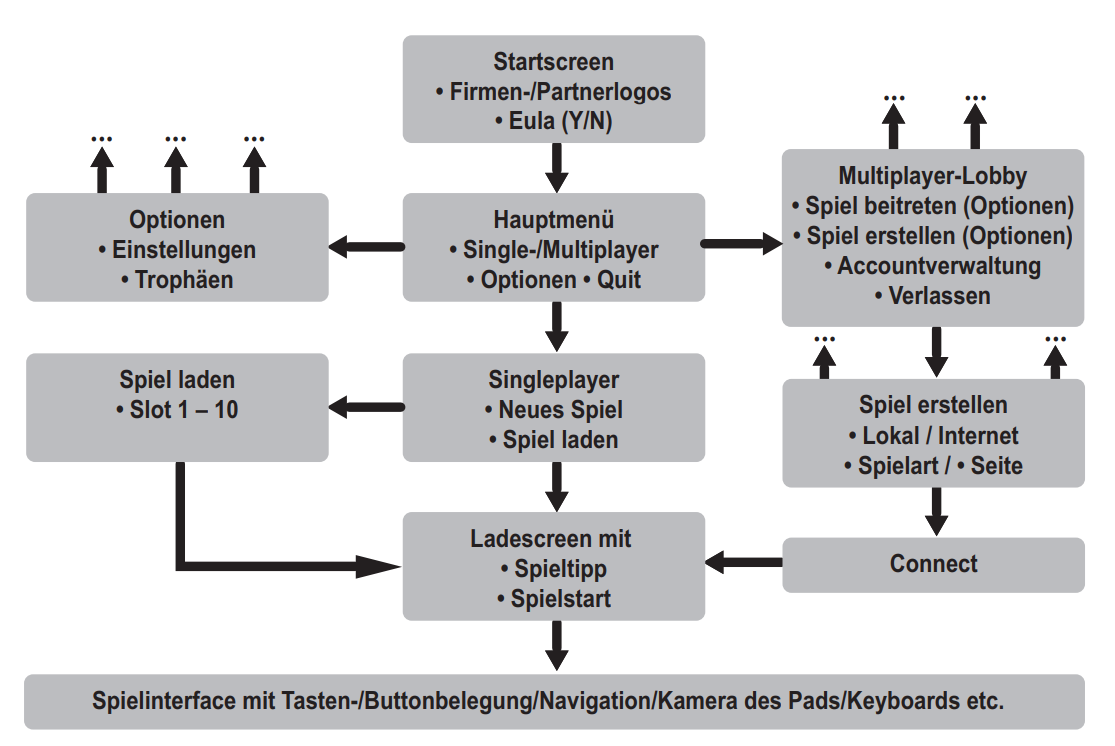
\includegraphics[width=0.6\textwidth]{chapters/03/images/Spielinterface.png}
  \caption{Ein Beispiel eines Dialogbaumes von einem Computerspiel.}
  \label{htl01}
\end{figure}

Der abgebildete Dialogbaum zeigt die verschiedenen Menüs und Screens die ein Computerspiel haben kann. Diese unterscheiden sich in den unterschiedlichen Arten von Spielen. Bei einem \bettergls{multiplayer}{2}-Spiel soll die Möglichkeit geboten werden, ein Spiel zu erstellen oder einem beizutreten. Während es bei einem \bettergls{singleplayer}{3} wichtig ist, Spielstände speichern und laden zu können.

\pagebreak

Das User Interface des Prototyps unterteilt sich in drei verschiedene Aspekte:

\begin{itemize}
    \item Hauptmenü
    \item User Interface während des Spieles
    \item Pausemenü
\end{itemize}

\noindent
Bei der Entscheidung, welche Komplexität das User Interface des Prototyps haben soll, fiel die Wahl auf ein simples Design. 
Das User Interface soll einerseits die Schlichtheit des eigentlichen Spieles wiederspiegeln und andererseits alle für das Spiel wichtigen Informationen darstellen.

\section{Gestaltung des Hauptmenüs}

Im Folgenden wird das Gestalten der Benutzeroberfläche für das Hauptmenü erläutert. 
Das Hauptmenü in der Spielentwicklung ist vergleichbar mit einem Türvorleger vor einer Haustür. Es soll das Willkommenschild für das eigentliche Spiel sein. 
Mithilfe dieses ersten Eindrucks ist es möglich zu erkennen, um welche Art von Spiel es sich handelt. Das \bettergls{theme}{1} des Spieles spiegelt sich in dem Design des Hintergrundes und in der Schriftart des Hauptmenüs wieder. Die Komplexität steht bei vielen Spielen in direkter Korrelation mit der Anzahl an Einstellungen in dem Hauptmenü.

\pagebreak

\subsection{Das Hauptmenü des Prototyps}

Das Hauptmenü des Prototyps besteht aus mehreren Komponenten. Die Hauptkomponente ist ein \bettergls{canvas}{1}. Diesem untergeordnet ist ein Bild, ein \bettergls{gameObject}{2} für das Hauptmenü und ein Game-Objekt für das Optionsmenü. Diese beiden Spiel-Objekte sind die eigentlichen Menüs, die dementsprechen ein- und ausgeblendet werden. Die Knöpfe, die der User betätigen kann, sind den Game-Objek<ten für das Hauptmenü und dem Optionsmenü untergeordnet. 

\subsubsection{Der Hintergrund}
Der Hintergrund des Hauptmenüs ist ein PNG von der \bettergls{skybox}{3} des Spiels. 
\subsubsection{Die Buttons}
Die Abbildungen \ref{htl02a} und \ref{htl02b} zeigen das Hauptmenü (links) und das Optionsmenü (rechts) des Prototyps. In dem Hauptmenü gibt es drei verschiedene Buttons: Play, Options and Quit. Play startet den Spielablauf, Options öffnet das Optionsmenü und Quit schließt das Spiel. In dem Optionsmenü befindet sich die Lautstärkenregelung. Der \glqq Back\grqq \space Button dient dazu zurück in das Hauptmenü zu kommen, befindet sich an letzter Stelle des Optionsmenüs.

\begin{figure}[H]
    \centering
    \begin{minipage}{0.4\textwidth}
        \centering
        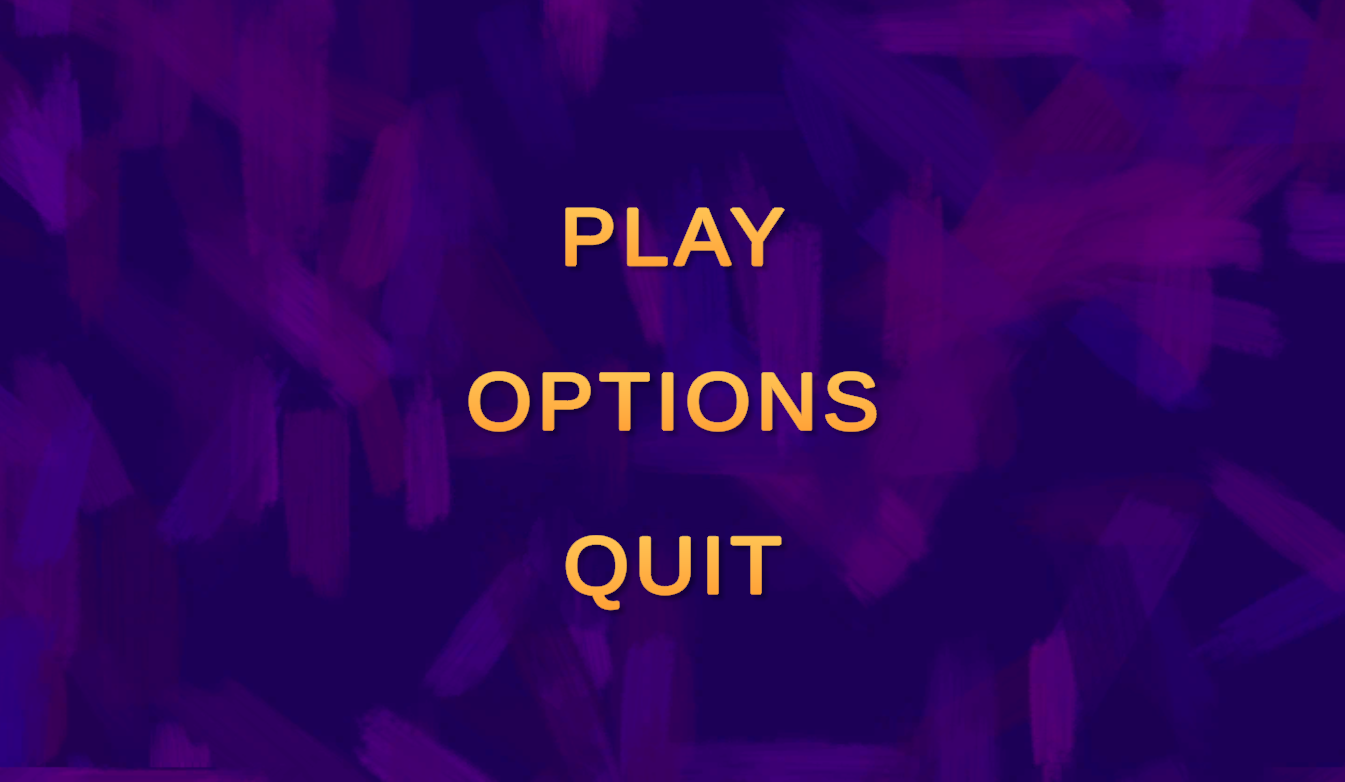
\includegraphics[width=\linewidth]{chapters/03/images/MainMenu.png}
        \caption{Das Hauptmenü des Prototyps.}
        \label{htl02a}
    \end{minipage}%
    \hspace{1cm}% Adjust the space here as needed
    \begin{minipage}{0.4\textwidth}
        \centering
        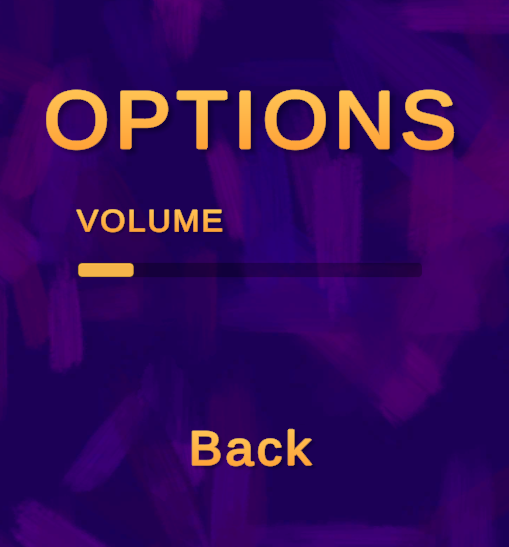
\includegraphics[width=\linewidth]{chapters/03/images/OptionsMainMenu.png}
        \caption{Das Optionsmenü des Prototyps.}
        \label{htl02b}
    \end{minipage}
\end{figure}

\section{Code behind des Menüs}

Der \bettergls{code-behind}{1} des Menüs ist sehr simpel gehalten und auch einfach zu verstehen.

% C#
\begin{lstlisting}[language=CSharp,caption={Main Menu Klasse.},label=code:mainmenu]
public class MainMenu : MonoBehaviour
{
    public void PlayGame()
    {
        var activeScene = SceneManager.GetActiveScene();
        SceneManager.LoadScene(activeScene.buildIndex + 1);
    }

    public void QuitGame()
    {
        Debug.Log("Quit");
        Application.Quit();
    }
}
\end{lstlisting}
Der SceneManager ist ein einfacher Weg mittels einer Art von \bettergls{statemachine}{2} eine Menüführung aufzubauen. In der nächsten Abbildung wird die Build-Reihenfolge der Scenes dargestellt.

\begin{center}
    \begin{figure}[h]
        \centering
        \includegraphics*[width=1\textwidth]{chapters/03/images/SceneManager.png}
        \caption{Der SceneManager in den Build Settings.}
        \label{htl04}
    \end{figure}
\end{center}

\noindent
Mittels der Code Zeile: 
% C#
\begin{lstlisting}[language=CSharp]
    SceneManager.LoadScene(activeScene.buildIndex + 1);
\end{lstlisting}
kann von der Menü Scene, die an der Stelle 0 ist zu der Projekt Scene, die an der Stelle 1 ist, gewechselt werden.

\pagebreak

\subsection{Die Funktion dem Button zuordnen}

In der nächsten Abbildung ist ein Ausschnitt der Properties des Play Buttons zu sehen. Bei der \verb+On Click ()+ Property wurde das \verb+MainMenu+ Skript hinzugefügt. Nachdem das Skript dort ausgewählt wurde, ist es möglich Methoden von diesem als Aktion für den Button auszuwählen. 

\begin{figure}[H]
    \centering
    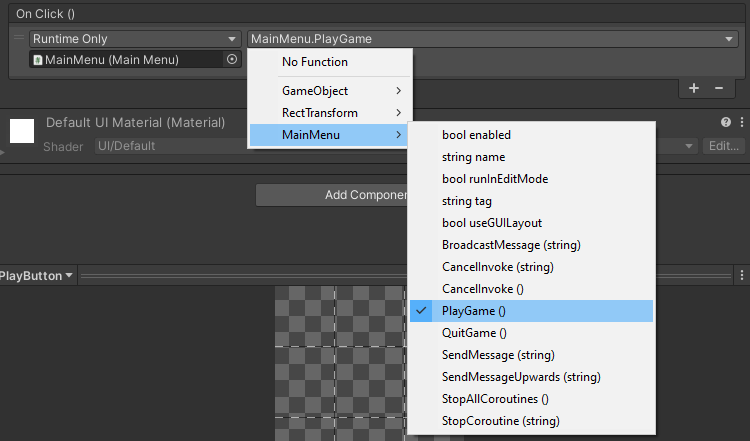
\includegraphics[width=0.6\textwidth]{chapters/03/images/PlayButton.png}
    \caption{Abbildung der Properties des Play Buttons.}
    \label{htl05}
\end{figure}

\section{Pausemenü und Game Over Screen}


Die Pause-Funktion ist ein wichtiger Teil eines Spiels, da sie den Spielern die Möglichkeit bietet, das Spiel zu pausieren, Einstellungen anzupassen oder sogar das Spiel zu verlassen, ohne den Fortschritt zu verlieren. Ebenso bedeutend ist der Game Over Screen, der dem Spieler nach einem Scheitern die Möglichkeit gibt, das Spiel neu zu starten oder komplett zu beenden.

\begin{figure}[H]
    \centering
    \begin{minipage}{0.4\textwidth}
        \centering
        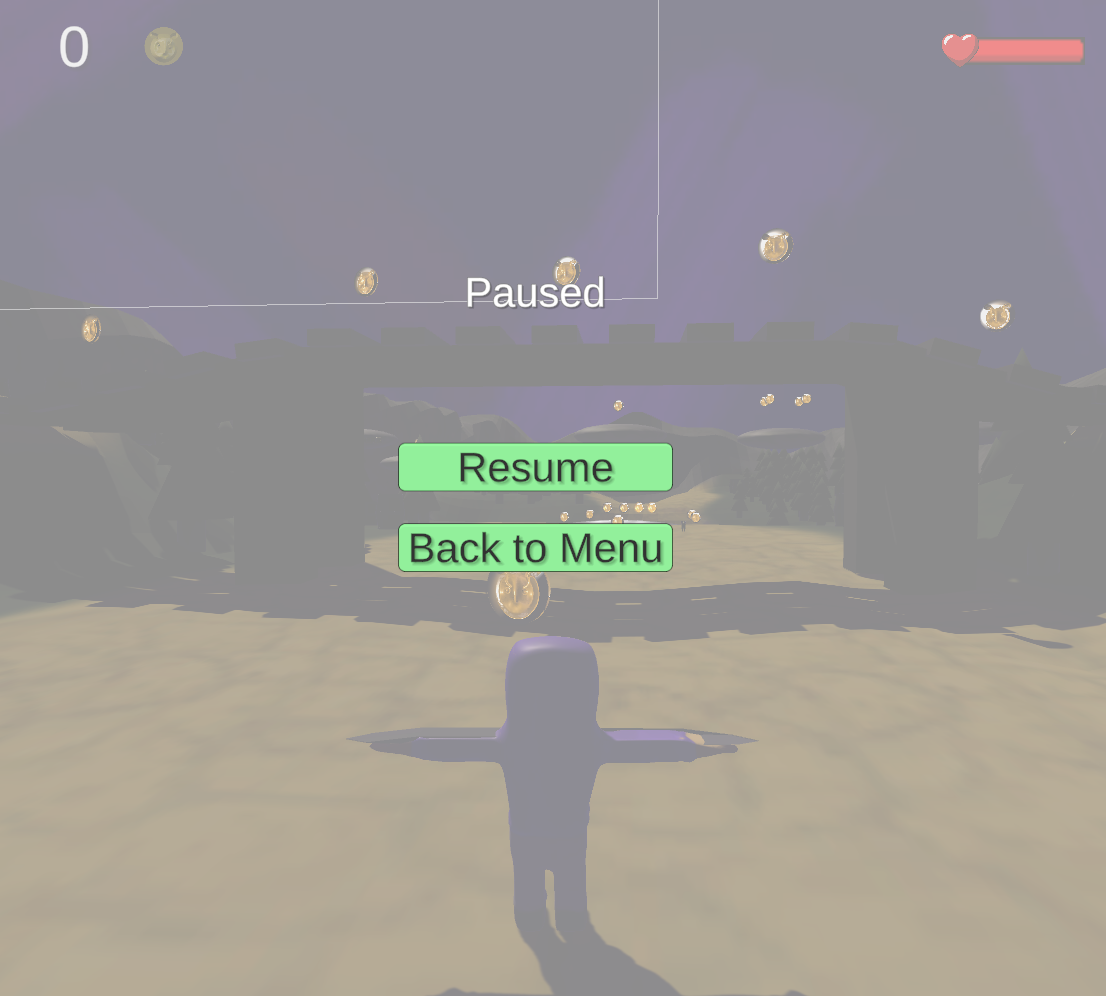
\includegraphics[width=\linewidth]{chapters/03/images/GamePaused.png}
        \caption{Das Game Paused UI des Prototypen.}
        \label{UI01}
    \end{minipage}
    \hspace{1cm}
    \begin{minipage}{0.4\textwidth}
        \centering
        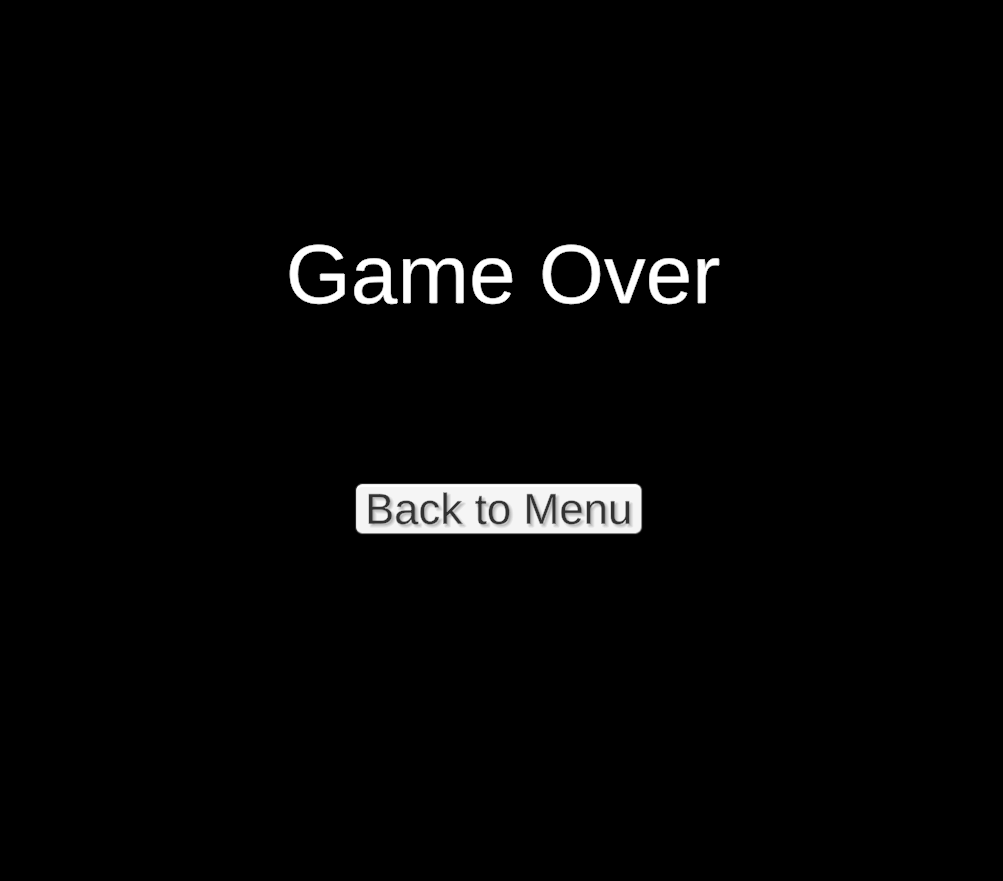
\includegraphics[width=\linewidth]{chapters/03/images/GameOver.png}
        \caption{Der Game Over Screen des Prototypen.}
        \label{UI02}
    \end{minipage}
\end{figure}



\section{Game UI und Spielmechanik-Anzeigen}

\begin{figure}[H]
    \centering
    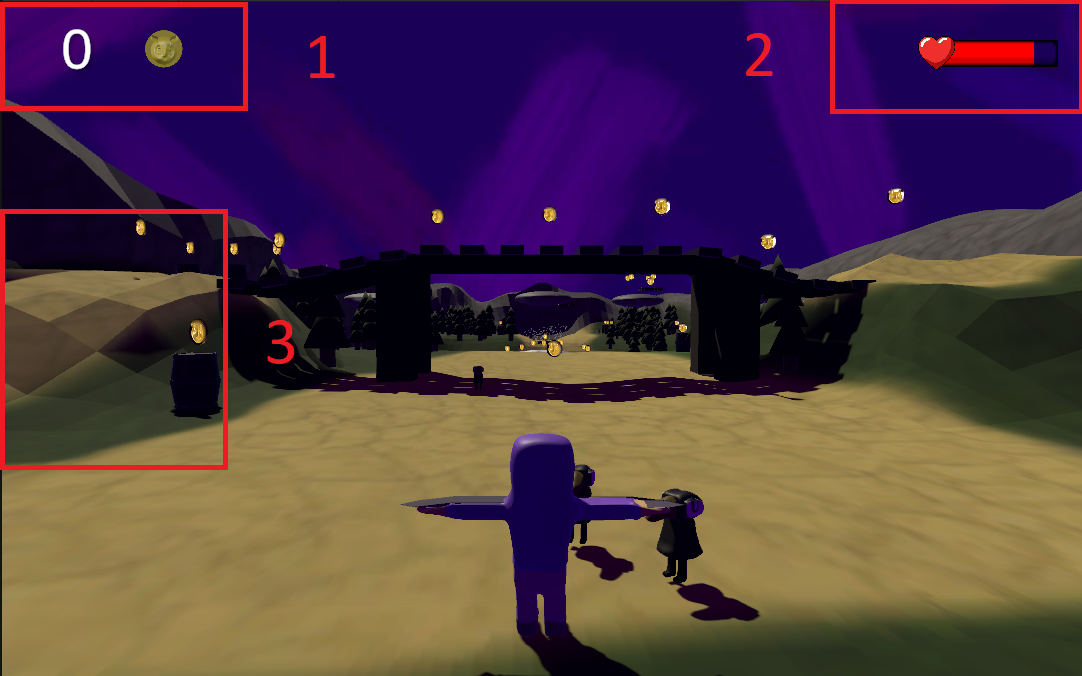
\includegraphics[width=0.8\textwidth]{chapters/03/images/GameUI.png}
    \caption{Das UI während des Spiels.}
    \label{htl03}
\end{figure}

\subsection{Eulenmünzen (1)}
Sammelobjekte, oder auch Collectibles gennant, gibt es in vielen Computerspielen. Jedoch bieten sie die unterschiedlichsten Funktionen. In PacMan ist das Sammeln von den Punkten teil des Spielziels. Verglichen zu Donkey Kong, wo das Sammeln von den Collectibles nicht verpflichtend ist. Aber es ist Teil von 101\% Vervollständigung des Spiels.
%https://donkeykong.fandom.com/wiki/Donkey_Kong_64#Gameplay

Als Sammelobjekt gibt es in dem Prototypen so gennante \glqq Eulenmünzen\grqq. Diese dienen ähnlich wie bei Donkey Kong als nicht verpflichtende Nebenaufgabe. Die Münzen schweben überall verstreut über die Welt des Prototypen. 

\subsection{Lebensanzeige (2)}

Eine Lebensanzeige in einem Computerspiel ist ein dezenter Hinweis darauf, dass der Spielcharakter sterblich ist. Schaden kann von Gegnern oder Fallen genommen werden.

In dem Prototypen wird die Lebensanzeige als roter Balken neben einem Herz dargestellt. Dieses Symbol befindet sich in der rechten oberen Ecke des Bildschirms. Lebensenergie wird abgezogen wenn die Spielfigur von einem Gegner getroffen wird oder in das \bettergls{void}{1} fällt.

\subsection{Steuerung (3)}
Die Idee war es die Steuerung auf dem User Interface darzustellen. Das ist ein einfacher Weg, das Spielkonzept dem Spieler näherzubringen. Ein gutes Beispiel dafür ist die Startwelt von Super Mario Odyssey. Dieses Spiel war auch eine große Inspiration für den Prototypen. 

%todo: level2 ui übergabe von wert... 67

\section{UI des zweiten Levels}

\begin{figure}[h]
    \centering
    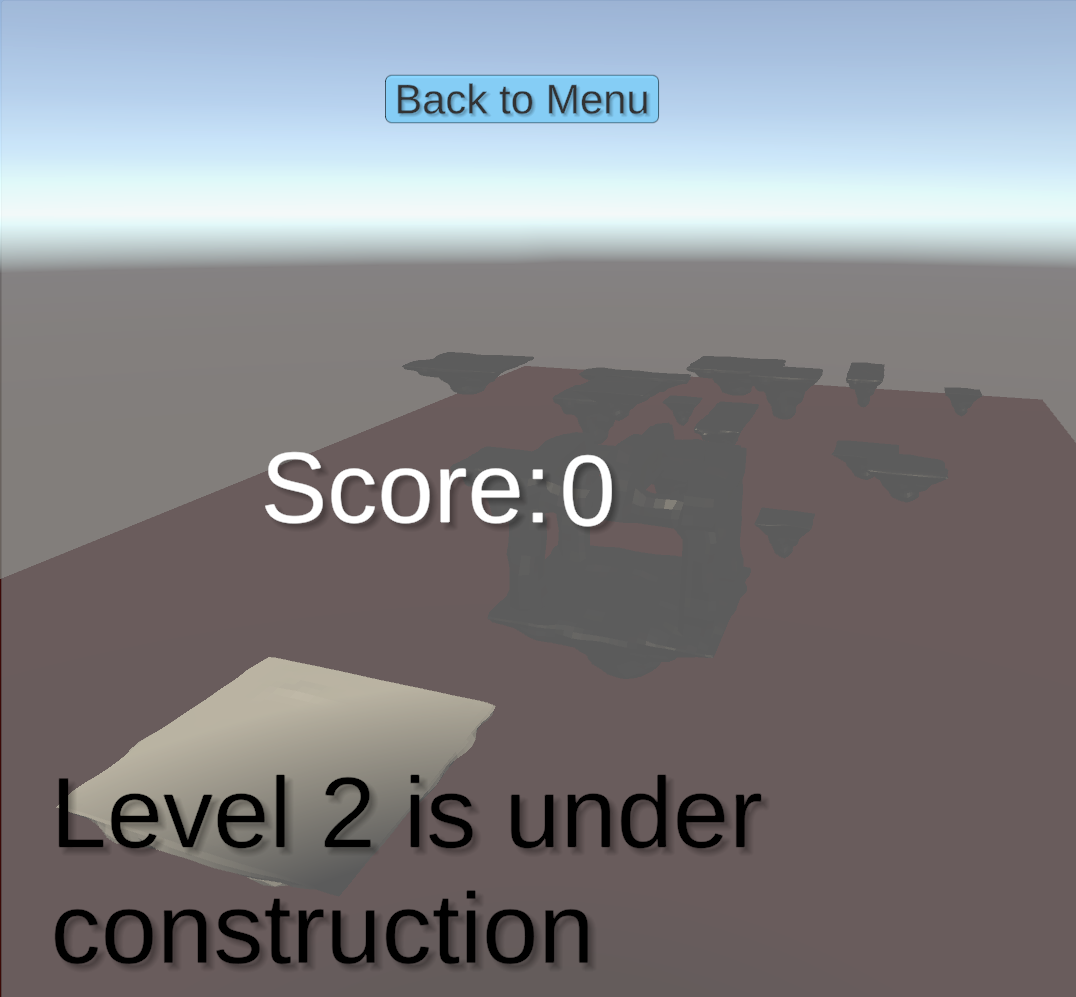
\includegraphics[width=0.6\textwidth]{chapters/04/images/V3/Level2Game.png}
    \caption{Der Endbildschirm des Prototypen.}
    \label{fig:UI20}
\end{figure}

\addcontentsline{toc}{chapter}{Spielkonzept} 
\addcontentsline{toc}{chapter}{Prototyp-Entwicklung}

\addcontentsline{toc}{chapter}{Tests und Qualitätssicherung?}
\addcontentsline{toc}{chapter}{Vermarktung und Veröffentlichung}
\addcontentsline{toc}{chapter}{Zusammenfassung und Ausblick}

\appendix

\newpage
\printnoidxglossaries

%\chapter*{Acknowledgements}
\addcontentsline{toc}{chapter}{Acknowledgements}

%\addcontentsline{toc}{chapter}{Listings}
%\lstlistoflistings

\addcontentsline{toc}{chapter}{List of Figures}
\listoffigures

\addcontentsline{toc}{chapter}{Bibliography}
\printbibliography

%
\chapter*{CV} \markboth{CV}{CV}
\addcontentsline{toc}{chapter}{CV}


\htlParagraph{Frieda Fröhlich}

\renewcommand{\arraystretch}{1.2}
\begin{tabularx}{1\textwidth}{@{} l X l @{}}

\emph{Geburtstag, Geburtsort:} & 01.01.1970, Braunau am Inn & 
\multirow{5}{2.5cm}{
    %\includegraphics[width=2.5cm]{./media/images/einstein.jpg}
} 
\\
\emph{Schulbildung:} & Volksschule \newline Hauptschule \newline HTL & \\
\emph{Praktika:} & Firmenname, Zeit, Tätigkeit & \\
\emph{Anschrift:} & Strasse Nummer\newline PLZ, Ort\newline Österreich & \\
\emph{E-Mail:} & frieda@froehlich.com & \\

\end{tabularx}
\\\\


\htlParagraph{Max Mustermann}

\begin{tabularx}{1\textwidth}{@{} l X l @{}}
\emph{Geburtstag, Geburtsort:} & 01.01.1970, Braunau am Inn & 
\multirow{5}{2.5cm}{
    %\includegraphics[width=2.5cm]{./media/images/einstein.jpg}
} 
\\
\emph{Schulbildung:} & Volksschule \newline Hauptschule \newline HTL & \\
\emph{Praktika:} & Firmenname, Zeit, Tätigkeit & \\
\emph{Anschrift:} & Strasse Nummer\newline PLZ, Ort\newline Österreich & \\
\emph{E-Mail:} & max@mustermann.com & \\

\end{tabularx}


\pagebreak
\htlParagraph{Max Mustermann}

\begin{tabularx}{1\textwidth}{@{} l X l @{}}
\emph{Geburtstag, Geburtsort:} & 01.01.1970, Braunau am Inn & 
\multirow{5}{2.5cm}{
    %\includegraphics[width=2.5cm]{./media/images/einstein.jpg}
} 
\\
\emph{Schulbildung:} & Volksschule \newline Hauptschule \newline HTL & \\
\emph{Praktika:} & Firmenname, Zeit, Tätigkeit & \\
\emph{Anschrift:} & Strasse Nummer\newline PLZ, Ort\newline Österreich & \\
\emph{E-Mail:} & max@mustermann.com & \\

\end{tabularx}
\chapter{Anhang}
\renewcommand{\arraystretch}{1}
\section{Betreuungsprotokolle} \markboth{Betreuungsprotokolle}{Betreuungsprotokolle}

% 111111111111111111111111111111111111111111111111111111111111111111111111111

\pagebreak

\noindent
\begin{tabular}{|m{0.2\textwidth}|m{0.6\textwidth}|m{0.2\textwidth}|}
\hline
\raisebox{-0.5\height}{
\includegraphics[width=1\linewidth]{media/images/htl-bildung-mit-zukunft.png}} 
&
\begin{center}
{\bfseries\sffamily\small HÖHERE TECHNISCHE BUNDES-LEHR- UND VERSUCHSANSTALT MÖDLING}\\[1ex]
{\small Höhere Lehranstalt für Elektronik und Technische Informatik\\
Kolleg für Informatik}
{\textcolor{gray}{bzw. Aufbaulehrgang für Informatik}}
\end{center} & 
\begin{center}
    {Reife- und Diplomprüfung}
\end{center} \\
\hline
\end{tabular}


\vspace*{20pt}
\subsection*{Betreuungsprotokoll zur Diplomarbeit \hfill lfd. Nr.: 1}
\vspace*{10pt}

\begin{tabular}{m{0.4\textwidth} m{0.4\textwidth}}
\textbf{Themenstellung:} & Unity Game Design und Development \\
\textbf{Kandidaten/Kandidatinnen:} & Schachinger Lukas, Usta Martin \\ \\
\textbf{Jahrgang:} & 2022/23 \\
\textbf{Betreuer/in:} & Hack Niklas \\
\textbf{Ort:} & Mödling \\
\textbf{Datum:} & 30.11.2022\\
\textbf{Zeit:} & 12:30 \\
\end{tabular}

\subsubsection*{Besprechungsinhalt:}
\begin{tabular}{|m{0.2\textwidth}|m{0.8\textwidth}|}
\hline
Name & Notiz \\
\hline
Usta, Schachinger & Anfang der Planung, Planung der Meilensteine, Einarbeitung des nächsten Meilensteins, Einrichten von DevOps Anfang der Umfeldanalyse \\
\hline
Usta & Aufgliederung der Meilensteine in Arbeitspackete,
Zuteilung der Arbeitspackete
Anfang der Umfeldanalyse von Designprogrammen,
2 von 3 wurden analysiert, Auswahlkriterien sind fertig\\
\hline
Schachinger & Aufgliederung der Meilensteine in Arbeitspackete, 
Zuteilung der Arbeitspakete
Anfang der Umfeldanalyse von Game Engines
1 von 3 wurden analysiert, Auswahlkriterien sind fertig\\
\hline
\end{tabular}

\subsubsection*{Aufgaben:}
\begin{tabular}{|m{0.2\textwidth}|m{0.6\textwidth}|m{0.2\textwidth}|}
\hline
Name & Notiz & zu erledigen bis \\
\hline
Usta & Fertigstellen der Umfeldanalysen 
Analyse von Designprogramm ZBrush & 12.12.2022 \\
\hline
Schachinger & Fertigstellen der Umfeldanalysen
Analyse von den Game Engines: Unreal, GoDot & 12.12.2022 \\
\hline
Usta & Grundgerüst Prototyp: 
Graphisches Leveldesign und erstellen der Low-Poly Assets
Implementierung der Charaktersteuerung & 18.12.2022 \\
\hline
Schachinger & Grundgerüst Prototyp: 
Implementierung der Bewegbaren Plattformen & 18.12.2022 \\
\hline
\end{tabular}

% 222222222222222222222222222222222222222222222222222222222222222222222222222

\pagebreak

\noindent
\begin{tabular}{|m{0.2\textwidth}|m{0.6\textwidth}|m{0.2\textwidth}|}
\hline
\raisebox{-0.5\height}{
\includegraphics[width=1\linewidth]{media/images/htl-bildung-mit-zukunft.png}} 
&
\begin{center}
{\bfseries\sffamily\small HÖHERE TECHNISCHE BUNDES-LEHR- UND VERSUCHSANSTALT MÖDLING}\\[1ex]
{\small Höhere Lehranstalt für Elektronik und Technische Informatik\\
Kolleg für Informatik}
{\textcolor{gray}{bzw. Aufbaulehrgang für Informatik}}
\end{center} & 
\begin{center}
    {Reife- und Diplomprüfung}
\end{center} \\
\hline
\end{tabular}


\vspace*{20pt}
\subsection*{Betreuungsprotokoll zur Diplomarbeit \hfill lfd. Nr.: 2}
\vspace*{10pt}

\begin{tabular}{m{0.4\textwidth} m{0.4\textwidth}}
\textbf{Themenstellung:} & Unity Game Design und Development \\
\textbf{Kandidaten/Kandidatinnen:} & Schachinger Lukas, Usta Martin \\ \\
\textbf{Jahrgang:} & 2022/23 \\
\textbf{Betreuer/in:} & Hack Niklas \\
\textbf{Ort:} & Mödling \\
\textbf{Datum:} & 19.12.2022 \\
\textbf{Zeit:} & 12:30 \\
\end{tabular}

\subsubsection*{Besprechungsinhalt:}
\begin{tabular}{|m{0.2\textwidth}|m{0.8\textwidth}|}
\hline
Name & Notiz \\
\hline
Usta & ZBrush noch nicht fertig analysiert \\
\hline
Usta & Leveldesign und Low-Poly fertig, Implementierung der Charaktersteuerung noch nicht fertig. \\
\hline
Schachinger & Umfeldanalyse für Unity und Unreal Engine fertig. Umfeldanalyse von GoDot noch nicht fertig. \\
\hline
Schachinger & Implementierung der bewegbaren Plattformen fertig. \\
\hline
\end{tabular}

\subsubsection*{Aufgaben:}
\begin{tabular}{|m{0.2\textwidth}|m{0.6\textwidth}|m{0.2\textwidth}|}
\hline
Name & Notiz & zu erledigen bis \\
\hline
Usta & ZBrush Umfeldanalyse fertigstellen & 28.02.2023 \\
\hline
Usta & Implementierung der Charaktersteuerung fertig & 28.02.2023 \\
\hline
Schachinger & GoDot Umfeldanalyse fertigstellen & 28.02.2023 \\
\hline
Schachinger, Usta & Planung des UI für eine optimale User Experience & 28.02.2023 \\
\hline
Schachinger & Aufbau und Erstellung einer Menu Führung & 28.02.2023 \\
\hline
Schachinger & Erstellung einer Statistikoberfläche & 28.02.2023 \\
\hline
\end{tabular}

% 333333333333333333333333333333333333333333333333333333333333333333333333333

\pagebreak

\noindent
\begin{tabular}{|m{0.2\textwidth}|m{0.6\textwidth}|m{0.2\textwidth}|}
\hline
\raisebox{-0.5\height}{
\includegraphics[width=1\linewidth]{media/images/htl-bildung-mit-zukunft.png}} 
&
\begin{center}
{\bfseries\sffamily\small HÖHERE TECHNISCHE BUNDES-LEHR- UND VERSUCHSANSTALT MÖDLING}\\[1ex]
{\small Höhere Lehranstalt für Elektronik und Technische Informatik\\
Kolleg für Informatik}
{\textcolor{gray}{bzw. Aufbaulehrgang für Informatik}}
\end{center} & 
\begin{center}
    {Reife- und Diplomprüfung}
\end{center} \\
\hline
\end{tabular}


\vspace*{20pt}
\subsection*{Betreuungsprotokoll zur Diplomarbeit \hfill lfd. Nr.: 3}
\vspace*{10pt}

\begin{tabular}{m{0.4\textwidth} m{0.4\textwidth}}
\textbf{Themenstellung:} & Unity Game Design und Development \\
\textbf{Kandidaten/Kandidatinnen:} & Schachinger Lukas, Usta Martin \\ \\
\textbf{Jahrgang:} & 2022/23 \\
\textbf{Betreuer/in:} & Hack Niklas \\
\textbf{Ort:} & Mödling \\
\textbf{Datum:} & 28.02.2023 \\
\textbf{Zeit:} & 12:30 \\
\end{tabular}

\subsubsection*{Besprechungsinhalt:}
\begin{tabular}{|m{0.2\textwidth}|m{0.8\textwidth}|}
\hline
Name & Notiz \\
\hline
Usta & ZBrush Umfeldanalyse muss noch überarbeitet werden. \\
\hline
Usta & Implementierung der Charaktersteuerung noch nicht fertiggestellt \\
\hline
Schachinger & GoDot Umfeldanalyse ist fertiggestellt. \\
\hline
Schachinger, Usta & Planung des UI für eine optimale User Experience. UI wurde neu erstellt, muss aber noch überarbeitet werden. \\
\hline
Schachinger & Aufbau und Erstellung einer Menu Führung noch nicht fertig, es fehlen Hauptmenü und Pausemenu.\\
\hline
Schachinger & Erstellung einer Statistikoberfläche fertiggestellt. \\
\hline
\end{tabular}

\subsubsection*{Aufgaben:}
\begin{tabular}{|m{0.2\textwidth}|m{0.6\textwidth}|m{0.2\textwidth}|}
\hline
Name & Notiz & zu erledigen bis \\
\hline
Usta & ZBrush Umfeldanalyse fertigstellen, anpassen auf das Layout & 20.03.2023 \\
\hline
Usta & Implementierung der Charaktersteuerung fertigstellen & 17.04.2023 \\
\hline
Schachinger & Planung des UI für eine optimale User Experience. UI überarbeiten und fertigstellen. & 20.03.2023 \\
\hline
Schachinger & Aufbau und Erstellung einer Menu Führung fertigstellen. & 17.04.2023 \\
\hline
Usta & Implementierung der High-Poly Assets & 31.05.2023 \\
\hline
Usta & Fertigstellung der Designaufgaben & 31.05.2023 \\
\hline
Schachinger & Fertigstellung der Programmieraufgaben & 31.05.2023 \\
\hline
\end{tabular}

% 444444444444444444444444444444444444444444444444444444444444444444444444444

\pagebreak

\noindent
\begin{tabular}{|m{0.2\textwidth}|m{0.6\textwidth}|m{0.2\textwidth}|}
\hline
\raisebox{-0.5\height}{
\includegraphics[width=1\linewidth]{media/images/htl-bildung-mit-zukunft.png}} 
&
\begin{center}
{\bfseries\sffamily\small HÖHERE TECHNISCHE BUNDES-LEHR- UND VERSUCHSANSTALT MÖDLING}\\[1ex]
{\small Höhere Lehranstalt für Elektronik und Technische Informatik\\
Kolleg für Informatik}
{\textcolor{gray}{bzw. Aufbaulehrgang für Informatik}}
\end{center} & 
\begin{center}
    {Reife- und Diplomprüfung}
\end{center} \\
\hline
\end{tabular}


\vspace*{20pt}
\subsection*{Betreuungsprotokoll zur Diplomarbeit \hfill lfd. Nr.: 4}
\vspace*{10pt}

\begin{tabular}{m{0.4\textwidth} m{0.4\textwidth}}
\textbf{Themenstellung:} & Unity Game Design und Development \\
\textbf{Kandidaten/Kandidatinnen:} & Schachinger Lukas, Usta Martin \\ \\
\textbf{Jahrgang:} & 2022/23 \\
\textbf{Betreuer/in:} & Hack Niklas \\
\textbf{Ort:} & Mödling \\
\textbf{Datum:} & 20.03.2023 \\
\textbf{Zeit:} & 10:30 \\
\end{tabular}

\subsubsection*{Besprechungsinhalt:}
\begin{tabular}{|m{0.2\textwidth}|m{0.8\textwidth}|}
\hline
Name & Notiz \\
\hline
Usta & ZBrush Umfeldanalyse fertiggestellt und auf ein einheitliches Layout angepasst. \\
\hline
Schachinger & UI noch nicht fertiggestellt Überarbeitung des Overlays (Münzen und Herzen) \\
\hline
\end{tabular}

\subsubsection*{Aufgaben:}
\begin{tabular}{|m{0.2\textwidth}|m{0.6\textwidth}|m{0.2\textwidth}|}
\hline
Name & Notiz & zu erledigen bis \\
\hline
Usta & Implementierung der Charaktersteuerung fertigstellen & 17.04.2023 \\
\hline
Schachinger & Überarbeitung des Overlays (Münzen und Herzen) & 17.04.2023 \\
\hline
Schachinger & Aufbau und Erstellung einer Menu Führung fertigstellen. & 17.04.2023 \\
\hline
Usta & Implementierung der High-Poly Assets & 31.05.2023 \\
\hline
Usta & Fertigstellung der Designaufgaben & 31.05.2023 \\
\hline
Schachinger & Fertigstellung der Designaufgaben & 31.05.2023 \\
\hline
\end{tabular}

% 555555555555555555555555555555555555555555555555555555555555555555555555555

\pagebreak

\noindent
\begin{tabular}{|m{0.2\textwidth}|m{0.6\textwidth}|m{0.2\textwidth}|}
\hline
\raisebox{-0.5\height}{
\includegraphics[width=1\linewidth]{media/images/htl-bildung-mit-zukunft.png}} 
&
\begin{center}
{\bfseries\sffamily\small HÖHERE TECHNISCHE BUNDES-LEHR- UND VERSUCHSANSTALT MÖDLING}\\[1ex]
{\small Höhere Lehranstalt für Elektronik und Technische Informatik\\
Kolleg für Informatik}
{\textcolor{gray}{bzw. Aufbaulehrgang für Informatik}}
\end{center} & 
\begin{center}
    {Reife- und Diplomprüfung}
\end{center} \\
\hline
\end{tabular}


\vspace*{20pt}
\subsection*{Betreuungsprotokoll zur Diplomarbeit \hfill lfd. Nr.: 5}
\vspace*{10pt}

\begin{tabular}{m{0.4\textwidth} m{0.4\textwidth}}
\textbf{Themenstellung:} & Unity Game Design und Development \\
\textbf{Kandidaten/Kandidatinnen:} & Schachinger Lukas, Usta Martin \\ \\
\textbf{Jahrgang:} & 2022/23 \\
\textbf{Betreuer/in:} & Hack Niklas \\
\textbf{Ort:} & Mödling \\
\textbf{Datum:} & 18.04.2023 \\
\textbf{Zeit:} & 10:00 \\
\end{tabular}

\subsubsection*{Besprechungsinhalt:}
\begin{tabular}{|m{0.2\textwidth}|m{0.8\textwidth}|}
\hline
Name & Notiz \\
\hline
Usta & Implementierung der Charaktersteuerung noch nicht fertiggestellt. \\
\hline
Schachinger & Überarbeitung des Overlays (Münzen und Herzen) fertiggestellt. \\
\hline
Schachinger & Pause und Quit Menu fertig, Spiel Hauptmenu noch nicht erstellt. \\
\hline
\end{tabular}

\subsubsection*{Aufgaben:}
\begin{tabular}{|m{0.2\textwidth}|m{0.6\textwidth}|m{0.2\textwidth}|}
\hline
Name & Notiz & zu erledigen bis \\
\hline
Schachinger & Spiel Hauptmenu erstellen. & 31.05.2023 \\
\hline
Usta & Charaktersteuerung muss überarbeitet werden. (Fähigkeiten und Text weiter verfassen) & 31.05.2023 \\
\hline
Usta & Implementierung der High-Poly Assets & 31.05.2023 \\
\hline
Usta & Fertigstellung der Designaufgaben & 31.05.2023 \\
\hline
Schachinger & Fertigstellung der Programmieraufgaben & 31.05.2023 \\
\hline
\end{tabular}

% 666666666666666666666666666666666666666666666666666666666666666666666666666

\pagebreak

\noindent
\begin{tabular}{|m{0.2\textwidth}|m{0.6\textwidth}|m{0.2\textwidth}|}
\hline
\raisebox{-0.5\height}{
\includegraphics[width=1\linewidth]{media/images/htl-bildung-mit-zukunft.png}} 
&
\begin{center}
{\bfseries\sffamily\small HÖHERE TECHNISCHE BUNDES-LEHR- UND VERSUCHSANSTALT MÖDLING}\\[1ex]
{\small Höhere Lehranstalt für Elektronik und Technische Informatik\\
Kolleg für Informatik}
{\textcolor{gray}{bzw. Aufbaulehrgang für Informatik}}
\end{center} & 
\begin{center}
    {Reife- und Diplomprüfung}
\end{center} \\
\hline
\end{tabular}


\vspace*{20pt}
\subsection*{Betreuungsprotokoll zur Diplomarbeit \hfill lfd. Nr.: 6}
\vspace*{10pt}

\begin{tabular}{m{0.4\textwidth} m{0.4\textwidth}}
\textbf{Themenstellung:} & Unity Game Design und Development \\
\textbf{Kandidaten/Kandidatinnen:} & Schachinger Lukas, Usta Martin \\ \\
\textbf{Jahrgang:} & 2022/23 \\
\textbf{Betreuer/in:} & Hack Niklas \\
\textbf{Ort:} & Mödling \\
\textbf{Datum:} & 31.05.2023 \\
\textbf{Zeit:} & 12:00 \\
\end{tabular}

\subsubsection*{Besprechungsinhalt:}
\begin{tabular}{|m{0.2\textwidth}|m{0.8\textwidth}|}
\hline
Name & Notiz \\
\hline
Usta & Charaktersteuerung muss noch überarbeitet werden. \\
\hline
Schachinger & Hauptmenu erstellt und implementiert. Settings müssen noch überarbeitet werden. \\
\hline
Usta & High Poly Assets erstellt muss noch implementiert werden. \\
\hline
Usta & Dokumentation über die Spiel Optimierung muss ausgebessert werden. \\
\hline
Schachinger & Programmieraufgaben sind noch nicht fertiggestellt. \\
\hline
Usta & Designaufgaben sind noch nicht fertiggestellt. \\
\hline
\end{tabular}

\subsubsection*{Aufgaben:}
\begin{tabular}{|m{0.2\textwidth}|m{0.6\textwidth}|m{0.2\textwidth}|}
\hline
Name & Notiz & zu erledigen bis \\
\hline
Schachinger & Settings im Pause Menu und im Haupt Menu überarbeiten. & 20.06.2023 \\
\hline
Usta & Charaktersteuerung muss weiter überarbeiten.  & 20.06.2023 \\
\hline
Usta & Implementierung der High-Poly Assets & 20.06.2023 \\
\hline
Usta & Fertigstellung der Designaufgaben & 20.06.2023 \\
\hline
Schachinger & Fertigstellung der Programmieraufgaben & 20.06.2023 \\
\hline
\end{tabular}

% 777777777777777777777777777777777777777777777777777777777777777777777777777

\pagebreak

\noindent
\begin{tabular}{|m{0.2\textwidth}|m{0.6\textwidth}|m{0.2\textwidth}|}
\hline
\raisebox{-0.5\height}{
\includegraphics[width=1\linewidth]{media/images/htl-bildung-mit-zukunft.png}} 
&
\begin{center}
{\bfseries\sffamily\small HÖHERE TECHNISCHE BUNDES-LEHR- UND VERSUCHSANSTALT MÖDLING}\\[1ex]
{\small Höhere Lehranstalt für Elektronik und Technische Informatik\\
Kolleg für Informatik}
{\textcolor{gray}{bzw. Aufbaulehrgang für Informatik}}
\end{center} & 
\begin{center}
    {Reife- und Diplomprüfung}
\end{center} \\
\hline
\end{tabular}


\vspace*{20pt}
\subsection*{Betreuungsprotokoll zur Diplomarbeit \hfill lfd. Nr.: 7}
\vspace*{10pt}

\begin{tabular}{m{0.4\textwidth} m{0.4\textwidth}}
\textbf{Themenstellung:} & Unity Game Design und Development \\
\textbf{Kandidaten/Kandidatinnen:} & Schachinger Lukas, Usta Martin \\ \\
\textbf{Jahrgang:} & 2022/23 \\
\textbf{Betreuer/in:} & Hack Niklas \\
\textbf{Ort:} & Mödling \\
\textbf{Datum:} & 20.06.2023 \\
\textbf{Zeit:} & 13:00 \\
\end{tabular}

\subsubsection*{Besprechungsinhalt:}
\begin{tabular}{|m{0.2\textwidth}|m{0.8\textwidth}|}
\hline
Name & Notiz \\
\hline
Schachinger & Menüführung muss noch finalisiert werden. \\
\hline
Schachinger & Finalisierung der Programmieraufgaben. \\
\hline
Usta & Charaktersteuerung muss noch finalisiert werden. \\
\hline
Usta & High-Poly Assets müssen noch fertiggestellt werden. \\
\hline
Usta & Finalisierung der Designaufgaben. \\
\hline
\end{tabular}

\subsubsection*{Aufgaben:}
\begin{tabular}{|m{0.2\textwidth}|m{0.6\textwidth}|m{0.2\textwidth}|}
\hline
Name & Notiz & zu erledigen bis \\
\hline
Schachinger & Fertigstellung der Menüführung. & 01.09.2023 \\
\hline
Schachinger & Finalisierung der Programmieraufgaben. & 01.09.2023 \\
\hline
Usta & Finalisierung der Charaktersteuerung.  & 01.09.2023 \\
\hline
Usta & Fertigstellung der High-Poly Assets. & 01.09.2023 \\
\hline
Usta & Finalisierung der Designaufgaben. & 01.09.2023 \\
\hline
\end{tabular}

\end{document}